% Double-anonymised build of main.tex (no author names, affiliations, contact details or funding).
\def\ANON{1}
% --- begin main.tex
% Main manuscript, Elsevier elsarticle (target: Computers in Biology and Medicine).
% Named build:       latexmk -pdf main.tex
% Blinded build:     latexmk -pdf manuscript_anonymised.tex   (defines \ANON before loading this file)
\documentclass[preprint,12pt,a4paper]{elsarticle}
\newif\ifanon
\ifdefined\ANON \anontrue \fi
\usepackage[T1]{fontenc}
\usepackage{newtxtext,newtxmath}
\usepackage[scaled=0.92]{helvet}
\usepackage{microtype}
\usepackage{amsmath}
\usepackage{booktabs,array,longtable,graphicx,float,placeins}
\usepackage{adjustbox}
\usepackage{enumitem}
\usepackage{xcolor}
\usepackage{url}
\usepackage{lineno}
\usepackage{tikz}
\usetikzlibrary{positioning,arrows.meta,calc,matrix}
\usepackage{pgfplots,pgfplotstable}
\pgfplotsset{compat=1.18}
\usepgfplotslibrary{groupplots}
\usepackage[colorlinks=true,linkcolor=blue!50!black,citecolor=blue!50!black,urlcolor=blue!50!black]{hyperref}
\biboptions{sort&compress}
\setlength{\parskip}{2pt}
% --- begin generated/numbers.tex
% auto-generated by experiments/report.py -- do not edit
\newcommand{\NMetabric}{2386}
\newcommand{\GThreeMetabric}{50.2}
\newcommand{\AgeMetabric}{61}
\newcommand{\NMsk}{1573}
\newcommand{\GThreeMsk}{67.6}
\newcommand{\AgeMsk}{52}
\newcommand{\NMbc}{207}
\newcommand{\GThreeMbc}{37.7}
\newcommand{\AgeMbc}{43}
\newcommand{\NSanger}{100}
\newcommand{\GThreeSanger}{51.0}
\newcommand{\AgeSanger}{55}
\newcommand{\NBroad}{59}
\newcommand{\GThreeBroad}{44.1}
\newcommand{\AgeBroad}{52}
\newcommand{\NBccrc}{63}
\newcommand{\GThreeBccrc}{88.9}
\newcommand{\AgeBccrc}{56}
\newcommand{\NTcga}{1072}
\newcommand{\GThreeTcga}{0.0}
\newcommand{\AgeTcga}{58}
\newcommand{\NDuke}{637}
\newcommand{\GThreeDuke}{32.5}
\newcommand{\AgeDuke}{52}
\newcommand{\NGradedTotal}{5025}
\newcommand{\NGradedCohorts}{7}
\newcommand{\NCohorts}{8}
\newcommand{\NAllTotal}{6097}
\newcommand{\NMetabricRecords}{2509}
\newcommand{\NMskSamples}{1918}
\newcommand{\NMskPatients}{1756}
\newcommand{\TauER}{-0.37}
\newcommand{\TauPR}{-0.31}
\newcommand{\TauHER}{+0.19}
\newcommand{\TauT}{+0.15}
\newcommand{\TauN}{+0.14}
\newcommand{\VHist}{0.18}
\newcommand{\RhoAge}{-0.12}
\newcommand{\NTests}{22}
\newcommand{\NSigTests}{20}
\newcommand{\BestIntModel}{Ordinal LR (prop. odds)}
\newcommand{\BestIntAuc}{0.725}
\newcommand{\BestIntAucLo}{0.709}
\newcommand{\BestIntAucHi}{0.743}
\newcommand{\MlrIntAuc}{0.725}
\newcommand{\OrdIntAuc}{0.725}
\newcommand{\XgbIntAuc}{0.723}
\newcommand{\KnnIntAuc}{0.715}
\newcommand{\IntAucSpread}{0.010}
\newcommand{\BestIntGThreeAuc}{0.752}
\newcommand{\IntAucMinR}{0.72}
\newcommand{\IntAucMaxR}{0.73}
\newcommand{\MlrIntFOne}{0.465}
\newcommand{\MajIntFOne}{0.223}
\newcommand{\MaxRepSd}{0.003}
\newcommand{\MaxDeltaInt}{0.008}
\newcommand{\MaxDeltaIntHi}{0.009}
\newcommand{\XgbDeltaInt}{+0.001}
\newcommand{\XgbDeltaIntLo}{-0.006}
\newcommand{\XgbDeltaIntHi}{+0.008}
\newcommand{\NSigBetterThanLr}{0}
\newcommand{\KnnDeltaInt}{-0.008}
\newcommand{\TabpfnStatus}{not run}
\newcommand{\TabpfnLimitation}{The pre-specified tabular foundation model (TabPFN) could not be run because its weights are distributed through a gated repository that was not reachable from the build environment; the code path is in place (\texttt{make tabpfn}). }
\newcommand{\BestExtModel}{Ordinal LR (prop. odds)}
\newcommand{\BestExtAuc}{0.713}
\newcommand{\BestExtAucLo}{0.688}
\newcommand{\BestExtAucHi}{0.737}
\newcommand{\MlrExtAuc}{0.710}
\newcommand{\XgbExtAuc}{0.711}
\newcommand{\MlrExtGThree}{0.727}
\newcommand{\NMskExt}{1573}
\newcommand{\CoreExtAucMin}{0.642}
\newcommand{\CoreExtAucMax}{0.797}
\newcommand{\LodoAucMin}{0.659}
\newcommand{\ExtAucMin}{0.64}
\newcommand{\ExtAucMax}{0.80}
\newcommand{\CoreMskMin}{0.64}
\newcommand{\CoreMskMax}{0.67}
\newcommand{\FullMskMin}{0.69}
\newcommand{\FullMskMax}{0.71}
\newcommand{\LodoAucMax}{0.778}
\newcommand{\NDukeExt}{637}
\newcommand{\MlrDukeAuc}{0.709}
\newcommand{\MlrDukeAucLo}{0.681}
\newcommand{\MlrDukeAucHi}{0.737}
\newcommand{\MlrDukeGThree}{0.779}
\newcommand{\FullDukeMin}{0.70}
\newcommand{\FullDukeMax}{0.72}
\newcommand{\MlrMskAucLo}{0.685}
\newcommand{\MlrMskAucHi}{0.734}
\newcommand{\NExtComparisons}{28}
\newcommand{\NExtSigBetter}{1}
\newcommand{\NExtSigWorse}{1}
\newcommand{\LeakMaxInfl}{+0.297}
\newcommand{\NpiHonest}{0.721}
\newcommand{\NpiLeaky}{0.972}
\newcommand{\SmoteHonestKnn}{0.652}
\newcommand{\SmoteLeakyKnn}{0.806}
\newcommand{\CompHonestDuke}{0.698}
\newcommand{\CompLeakyDuke}{0.995}
\newcommand{\CompHonest}{0.696}
\newcommand{\CompLeaky}{0.962}
\newcommand{\RecHonestKnn}{0.544}
\newcommand{\RecLeakyKnn}{0.579}
\newcommand{\CalIntMskRaw}{+0.99}
\newcommand{\CalSlopeMskRaw}{1.03}
\newcommand{\CalIntMskRec}{+0.00}
\newcommand{\CalSlopeInt}{1.00}
\newcommand{\CalSlopeIntXgb}{1.02}
\newcommand{\PrevMsk}{0.68}
\newcommand{\PredMsk}{0.47}
\newcommand{\CalIntDukeRaw}{-1.02}
\newcommand{\CalSlopeDukeRaw}{0.96}
\newcommand{\CalIntDukeRec}{+0.00}
\newcommand{\PrevDuke}{0.32}
\newcommand{\PredDuke}{0.52}
\newcommand{\CalSlopeMskXgb}{1.03}
\newcommand{\DcaLoInt}{0.26}
\newcommand{\DcaHiInt}{0.85}
\newcommand{\DcaLoExt}{0.63}
\newcommand{\DcaHiExt}{0.85}
\newcommand{\DcaLoDuke}{0.19}
\newcommand{\DcaHiDuke}{0.64}
\newcommand{\ShapAgree}{7 of 7}
\newcommand{\ShapTop}{ER positive}
\newcommand{\ShapSecond}{T category}
\newcommand{\OrER}{0.17}
\newcommand{\OrERlo}{0.12}
\newcommand{\OrERhi}{0.24}
\newcommand{\OrILC}{0.41}
\newcommand{\OrILClo}{0.28}
\newcommand{\OrILChi}{0.57}
\newcommand{\OrHer}{1.83}
\newcommand{\NOrdinal}{1800}
\newcommand{\RwGThreeMet}{60.9}
\newcommand{\RwGThreeMetLo}{58.5}
\newcommand{\RwGThreeMetHi}{63.0}
\newcommand{\ObsGThreeMet}{50.6}
\newcommand{\RwGOneMet}{6.2}
\newcommand{\RwGTwoMet}{32.9}
\newcommand{\EssMet}{1088}
\newcommand{\EssRedPct}{42}
\newcommand{\PredGThreeMet}{59.1}
\newcommand{\OverPredPP}{22}
\newcommand{\NRakedMet}{1861}
\newcommand{\AucUnwMet}{0.727}
\newcommand{\AucWMet}{0.790}
\newcommand{\RwGThreeMsk}{77.3}
\newcommand{\ObsGThreeMsk}{67.6}
\newcommand{\AucWMsk}{0.766}
\newcommand{\RwGThreeDuke}{42.1}
\newcommand{\ObsGThreeDuke}{32.5}
\newcommand{\RwGThreeMetB}{57.3}
\newcommand{\RwGThreeMetBLo}{54.6}
\newcommand{\RwGThreeMetBHi}{60.0}
\newcommand{\SaudiGThreeB}{48.8}
\newcommand{\PoolGThree}{44.7}
\newcommand{\PoolGThreeLo}{37.2}
\newcommand{\PoolGThreeHi}{52.5}
\newcommand{\PoolK}{3}
\newcommand{\PoolN}{908}
\newcommand{\PoolGThreeAll}{42.1}
\newcommand{\PoolGThreeAllLo}{34.5}
\newcommand{\PoolGThreeAllHi}{50.0}
\newcommand{\AgeSensMin}{60.5}
\newcommand{\AgeSensMax}{61.3}
\newcommand{\AgeSensLo}{40}
\newcommand{\AgeSensHi}{60}
\newcommand{\RwGThreeAllMin}{35.9}
\newcommand{\ShiftMin}{+9.6}
\newcommand{\ShiftMax}{+10.3}
\newcommand{\ObsGThreeMin}{32.5}
\newcommand{\ObsGThreeMax}{67.6}
\newcommand{\RwGThreeKMin}{42.1}
\newcommand{\RwGThreeKMax}{77.3}
\newcommand{\SaudiGThreeA}{36.7}
\newcommand{\RwGThreeAllMax}{77.3}
\newcommand{\MIDiffMax}{0.003}
\newcommand{\MIMlrAuc}{0.724}
\newcommand{\MIXgbAuc}{0.726}
\newcommand{\NComplete}{1800}
\newcommand{\CCMlrAuc}{0.729}
\newcommand{\MIm}{20}
\newcommand{\DukeClinAuc}{0.694}
\newcommand{\DukeClinAucLo}{0.663}
\newcommand{\DukeClinAucHi}{0.727}
\newcommand{\DukeClinGThree}{0.769}
\newcommand{\DukeRadAuc}{0.608}
\newcommand{\DukeRadAucLo}{0.575}
\newcommand{\DukeRadAucHi}{0.645}
\newcommand{\DukeRadGThree}{0.667}
\newcommand{\DukeFusAuc}{0.648}
\newcommand{\DukeFusAucLo}{0.618}
\newcommand{\DukeFusAucHi}{0.685}
\newcommand{\DukeFusGThree}{0.731}
\newcommand{\DukeRadDelta}{-0.085}
\newcommand{\DukeRadDeltaLo}{-0.126}
\newcommand{\DukeRadDeltaHi}{-0.045}
\newcommand{\DukeFusDelta}{-0.045}
\newcommand{\DukeFusDeltaLo}{-0.077}
\newcommand{\DukeFusDeltaHi}{-0.011}
\newcommand{\NDukeRad}{637}
\newcommand{\SSRequired}{4477}
\newcommand{\SSAvailable}{2386}
\newcommand{\SSParams}{10}
\newcommand{\SSMet}{not met}
\newcommand{\LjBest}{0.636}
\newcommand{\NLj}{286}
\newcommand{\Repeats}{10}
\newcommand{\Folds}{5}
\newcommand{\InnerFolds}{3}
\newcommand{\Boot}{2000}
\newcommand{\Seed}{20261017}
\newcommand{\TransportBoot}{500}
\newcommand{\RadRepeats}{10}
% --- end generated/numbers.tex

% --- begin figures/pgfstyle.tex
% Shared pgfplots style. Data come from generated/data/*.csv (written by experiments/report.py).
\definecolor{cA}{HTML}{2A78D6}\definecolor{cB}{HTML}{EB6834}\definecolor{cC}{HTML}{1BAF7A}\definecolor{cD}{HTML}{6250D6}
\definecolor{gI}{HTML}{B9D3F2}\definecolor{gII}{HTML}{5D98DE}\definecolor{gIII}{HTML}{174F94}
\definecolor{inkb}{HTML}{52514E}\definecolor{gridc}{HTML}{E4E3DF}
\pgfplotstableset{col sep=semicolon}
\pgfplotsset{
  table/col sep=semicolon,
  bcbase/.style={font=\sffamily\scriptsize, axis line style={inkb}, tick style={inkb},
    major grid style={gridc}, tick align=outside, axis x line*=bottom, axis y line*=left,
    legend style={draw=none, fill=none, font=\sffamily\scriptsize}, legend cell align=left},
  dotci/.style={only marks, mark=*, mark size=1.6pt, #1, error bars/.cd, x dir=both, x explicit,
    error bar style={#1, line width=1pt}, error mark=none},
}
\newcommand{\gdata}[1]{generated/data/#1.csv}
% --- end figures/pgfstyle.tex

\newcommand{\tabfit}[1]{\resizebox{\linewidth}{!}{#1}}
% repository link: replace with the anonymous mirror for review and the public URL/DOI after acceptance
\newcommand{\CodeURL}{\url{https://anonymous.4open.science/r/bc-grade-opendata}}
\journal{Computers in Biology and Medicine}

\begin{document}
\ifanon\linenumbers\fi

\begin{frontmatter}
\title{Predicting breast cancer grade from routine clinical data: an open multi-cohort study with transport to Saudi patients}

\ifanon
\author{[Author details removed for double-anonymised review]}
\else
\IfFileExists{authors.tex}{\input{authors.tex}}{% --- begin authors_placeholder.tex
% Placeholder used in the public/anonymous repository; the submission files carry the real author block.
\author{[Author details withheld for double-anonymised review]}
% --- end authors_placeholder.tex
}
\fi

% --- begin sections/abstract.tex
\begin{abstract}
\textbf{Background:} Histological grade guides breast cancer treatment but is assigned only after
tissue examination and is moderately reproducible. It is unknown how much of grade the routine record
carries, whether such models transport, and what they predict for Saudi patients.
\textbf{Methods:} We combined \NGradedTotal{} graded invasive breast cancers from \NGradedCohorts{}
public cohorts into one data model. Seven models, from a baseline to gradient boosting, were
developed in METABRIC (\NMetabric{} patients) with nested cross-validation and compared with
logistic regression. Frozen models were validated in five external cohorts. We assessed
discrimination, calibration and utility, measured leakage, tested 529 MRI radiomic features, and
re-weighted the cohorts to published Saudi case-mix.
\textbf{Results:} All learned models reached a macro-AUC of \IntAucMinR--\IntAucMaxR{} internally;
XGBoost did not beat logistic regression (difference \XgbDeltaInt, 95\% CI \XgbDeltaIntLo{} to
\XgbDeltaIntHi). External macro-AUCs were \FullMskMin--\FullMskMax{} and \FullDukeMin--\FullDukeMax{}
in the two full-feature cohorts. Calibration slopes stayed near one, but the models under-predicted
grade~3 in one cohort and over-predicted it in another; an intercept update corrected both. Leakage
shortcuts inflated macro-AUC by up to \LeakMaxInfl. Radiomics did not improve on clinical variables.
Saudi case-mix raised each cohort's grade-3 share by \ShiftMin{} to \ShiftMax{} points, yet a
METABRIC model would predict \PredGThreeMet\% grade~3 against \SaudiGThreeA\% published.
\textbf{Conclusions:} Routine variables predict grade moderately and consistently. Logistic
regression is sufficient, but local recalibration is essential. Western-trained models would
over-predict high-grade disease in Saudi patients.
\end{abstract}
% --- end sections/abstract.tex


\begin{keyword}
breast cancer \sep histological grade \sep clinical prediction model \sep external validation \sep
calibration \sep data leakage \sep radiomics \sep transportability \sep Saudi Arabia \sep TRIPOD+AI
\end{keyword}
\end{frontmatter}

% --- begin sections/introduction.tex
\section{Introduction}\label{sec:intro}

Histological grade is one of the strongest prognostic factors in invasive breast cancer. The
Nottingham (Elston--Ellis) system scores tubule formation, nuclear pleomorphism and mitotic count,
and the resulting grade of 1, 2 or 3 predicts survival independently of tumour size and nodal
status~\citep{elston1991grade,rakha2008nhg,rakha2010grade}. Grade has two practical weaknesses.
First, it is only available after a pathologist has examined tissue. Second, it is only moderately
reproducible: agreement between pathologists typically reaches a $\kappa$ of 0.5--0.7
\citep{boiesen2000grading,longacre2006interobserver}, grading rates differ between laboratories in
national data~\citep{vandooijeweert2020variation}, and the large intermediate group, grade~2, is
prognostically mixed~\citep{sotiriou2006ggi,vandooijeweert2022grading}.

Every patient record, however, already contains variables that are linked to grade: age, menopausal
status, oestrogen receptor (ER), progesterone receptor (PR) and HER2 status, histological type,
tumour size and nodal status. If these variables predict grade reliably, a simple model could fill
gaps in registry and trial data, flag records whose assigned grade is unlikely given the rest of the
record, and provide the baseline that image-based grading tools should beat. Recent work has moved
straight to images, predicting grade from whole-slide images with deep learning and pathology
foundation models~\citep{wang2022deepgrade,kim2025grade,chen2024uni} and from MRI
radiomics~\citep{wang2022duke,wang2026dcemrigrade}. We found no study that measured, on open data
from several countries, how much grade the routine record already carries.

\paragraph{Problem statement}
Three gaps prevent a reliable answer.
\begin{enumerate}[leftmargin=*,itemsep=1pt,topsep=2pt]
\item \emph{No transparent baseline.} Published grade-prediction studies are mostly single-centre,
rarely validate their models externally, and seldom report calibration, which is the property that
most often fails when a model moves to a new hospital~\citep{vancalster2019calibration,riley2024evalpart2}.
It is also unclear whether flexible machine-learning methods add anything over regression, which
systematic reviews suggest they usually do not~\citep{christodoulou2019lr}.
\item \emph{Hidden leakage.} Public breast cancer datasets include variables that contain grade by
construction, such as the Nottingham Prognostic Index and the three Nottingham component scores.
Using them as predictors, or fitting preprocessing steps before splitting the data, lets information
about the outcome reach the model and inflates performance~\citep{kapoor2023leakage,varoquaux2022failures,rosenblatt2024leakage}.
The size of this inflation for grade prediction has not been measured.
\item \emph{Unknown transport to Saudi patients.} Breast cancer is the most common cancer in Saudi
women; its age-standardised incidence rose from 11.8 to 29.7 per 100{,}000 between 2001 and 2017,
when it accounted for 30.9\% of female cancers~\citep{basudan2022registry}. Patients in Arab
countries are younger and more often have hormone-receptor-negative or HER2-positive
disease than patients in Western cohorts~\citep{najjar2010arab,chouchane2013arab,elkum2007young,altamimi2010saudi}.
No grade-labelled patient-level dataset from the region is openly available, and local studies are
based on single-centre records that cannot be
shared~\citep{kussaibi2021saudi,durrani2025healthcare}. It is therefore unknown whether models built
on Western data would give correct predictions for Saudi patients~\citep{debray2015framework,steingrimsson2023transport}.
\end{enumerate}

\paragraph{Research questions}
We address these gaps with openly downloadable data only, so that every result can be reproduced by
any reader. We ask:
\textbf{RQ1}, how strongly is grade associated with each routine variable?
\textbf{RQ2}, how well do models of increasing flexibility predict grade, within the development
cohort and in independent cohorts from other countries, and are they well calibrated?
\textbf{RQ3}, how much do common analytic shortcuts inflate apparent performance?
\textbf{RQ4}, do MRI radiomic features add to the routine record?
\textbf{RQ5}, what would Western-developed models predict for patients with a Saudi case-mix?

\paragraph{Contributions}
\begin{enumerate}[leftmargin=*,itemsep=1pt,topsep=2pt]
\item A harmonised, checksummed data model of \NGradedTotal{} grade-labelled invasive breast cancers
from \NGradedCohorts{} public cohorts on three continents, built with explicit rules that exclude
in-situ disease, keep lobular and ductal carcinoma separate and allow one record per patient
(Figure~\ref{fig:framework}).
\item A model comparison that follows TRIPOD+AI~\citep{collins2024tripodai}: seven models from a
prevalence baseline to gradient boosting, nested cross-validation, multiple imputation, paired
comparisons with logistic regression, validation in five external cohorts and across datasets,
calibration with model updating, and decision curves.
\item To our knowledge, the first measurement, on the same data and models, of how much four common leakage
shortcuts inflate apparent performance for grade prediction.
\item A head-to-head test of 529 MRI radiomic features against the routine record in the same
patients.
\item A transport analysis that re-weights open cohorts to published Saudi hospital series and shows
what Western-developed models would imply for Saudi patients.
\end{enumerate}
% --- end sections/introduction.tex

% --- begin sections/methods.tex
\section{Methods}\label{sec:methods}

\subsection{Study design and reporting}
This is a secondary analysis of de-identified, publicly released data. We report the prediction
analysis according to TRIPOD+AI~\citep{collins2024tripodai} and the descriptive analysis according to
STROBE~\citep{vonelm2007strobe}; the completed TRIPOD+AI checklist is in Supplementary
Table~\ref{tab:tripod}. Figure~\ref{fig:framework} shows the study framework in three lanes: data
preparation (A), model development and validation (B), and the checks that test the results (C).
Before running any experiment, we fixed the feature sets, models, metrics, expected directions of
effect and re-weighting targets in a configuration file (random seed \Seed). All tables, figures
and numbers in this paper are generated directly from the results files by code.

\begin{figure*}[t]\centering
\resizebox{\linewidth}{!}{% --- begin figures/fig_framework.tex
% Figure 1 -- study framework (three lanes). Counts are macros from generated/numbers.tex.
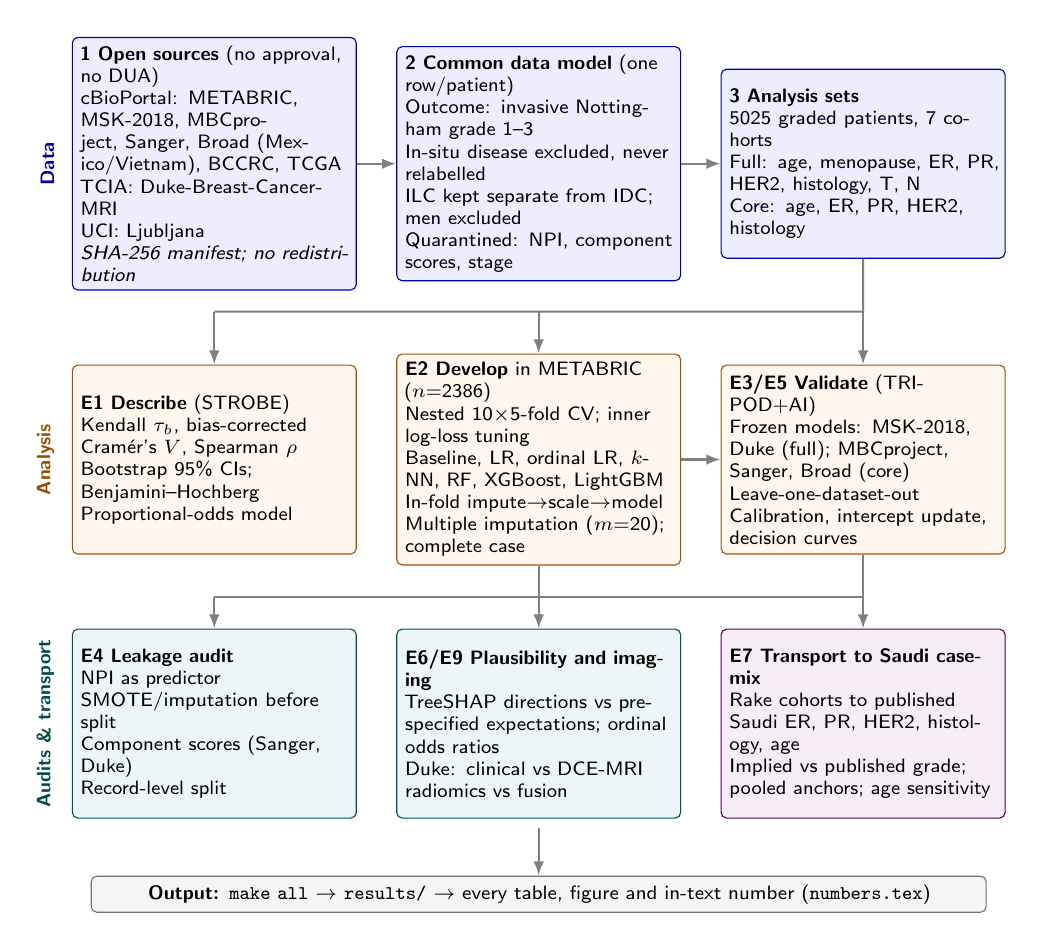
\begin{tikzpicture}[
  font=\sffamily\scriptsize,
  box/.style={draw=#1!65!black, fill=#1!7, rounded corners=2pt, align=left, inner sep=3pt,
              text width=0.28\linewidth, minimum height=24mm},
  lane/.style={font=\sffamily\scriptsize\bfseries, text=#1!60!black, rotate=90, anchor=south},
  arr/.style={-{Latex[length=1.8mm]}, thick, draw=black!50},
  bus/.style={thick, draw=black!50},
]
\matrix (m) [row sep=8mm, column sep=5mm, ampersand replacement=\&] {
\node[box=blue] (src) {\textbf{1 Open sources} (no approval, no DUA)\\
  cBioPortal: METABRIC, MSK-2018, MBCproject, Sanger, Broad (Mexico/Vietnam), BCCRC, TCGA\\
  TCIA: Duke-Breast-Cancer-MRI\\
  UCI: Ljubljana\\
  \emph{SHA-256 manifest; no redistribution}}; \&
\node[box=blue] (cdm) {\textbf{2 Common data model} (one row/patient)\\
  Outcome: invasive Nottingham grade 1--3\\
  In-situ disease excluded, never relabelled\\
  ILC kept separate from IDC; men excluded\\
  Quarantined: NPI, component scores, stage}; \&
\node[box=blue] (fs) {\textbf{3 Analysis sets}\\
  \NGradedTotal{} graded patients, \NGradedCohorts{} cohorts\\
  Full: age, menopause, ER, PR, HER2, histology, T, N\\
  Core: age, ER, PR, HER2, histology}; \\
\node[box=orange] (e1) {\textbf{E1 Describe} (STROBE)\\
  Kendall $\tau_b$, bias-corrected Cram\'er's $V$, Spearman $\rho$\\
  Bootstrap 95\% CIs; Benjamini--Hochberg\\
  Proportional-odds model}; \&
\node[box=orange] (e2) {\textbf{E2 Develop} in METABRIC ($n$=\NMetabric)\\
  Nested \Repeats$\times$\Folds-fold CV; inner log-loss tuning\\
  Baseline, LR, ordinal LR, $k$-NN, RF, XGBoost, LightGBM\\
  In-fold impute$\to$scale$\to$model\\
  Multiple imputation ($m$=\MIm); complete case}; \&
\node[box=orange] (e3) {\textbf{E3/E5 Validate} (TRIPOD+AI)\\
  Frozen models: MSK-2018, Duke (full); MBCproject, Sanger, Broad (core)\\
  Leave-one-dataset-out\\
  Calibration, intercept update, decision curves}; \\
\node[box=teal] (e4) {\textbf{E4 Leakage audit}\\
  NPI as predictor\\ SMOTE/imputation before split\\ Component scores (Sanger, Duke)\\ Record-level split}; \&
\node[box=teal] (e6) {\textbf{E6/E9 Plausibility and imaging}\\
  TreeSHAP directions vs pre-specified expectations; ordinal odds ratios\\
  Duke: clinical vs DCE-MRI radiomics vs fusion}; \&
\node[box=violet] (e7) {\textbf{E7 Transport to Saudi case-mix}\\
  Rake cohorts to published Saudi ER, PR, HER2, histology, age\\
  Implied vs published grade; pooled anchors; age sensitivity}; \\
};
\node[draw=black!55, fill=black!4, rounded corners=2pt, anchor=north, inner sep=3pt, align=center,
      text width=0.92\linewidth] (out) at ([yshift=-6mm]m.south)
  {\textbf{Output:} \texttt{make all} $\to$ \texttt{results/} $\to$ every table, figure and in-text number (\texttt{numbers.tex})};
\draw[arr] (src) -- (cdm); \draw[arr] (cdm) -- (fs);
% bus from data lane to analysis lane
\coordinate (b1) at ($(fs.south)!0.5!(e3.north)$);
\draw[bus] (fs.south) -- (b1) -- (b1 -| e1.north);
\foreach \n in {e1,e2,e3} \draw[arr] (b1 -| \n.north) -- (\n.north);
\draw[arr] (e2) -- (e3);
% bus from analysis lane to audit lane
\coordinate (b2) at ($(e2.south)!0.5!(e6.north)$);
\draw[bus] (e2.south) -- (b2); \draw[bus] (b2 -| e4.north) -- (b2 -| e7.north);
\draw[bus] (e3.south) -- (b2 -| e3.south);
\foreach \n in {e4,e6,e7} \draw[arr] (b2 -| \n.north) -- (\n.north);
\draw[arr] (m.south) -- (out.north);
\node[lane=blue]   at ([xshift=-1mm]src.west) {Data};
\node[lane=orange] at ([xshift=-1mm]e1.west)  {Analysis};
\node[lane=teal]   at ([xshift=-1mm]e4.west)  {Audits \& transport};
\end{tikzpicture}
% --- end figures/fig_framework.tex
}
\caption{Study framework. \textbf{A}, open data are downloaded with checksums and mapped to one row
per patient under four harmonisation rules; variables that contain grade are set aside.
\textbf{B}, associations are measured with statistics suited to each variable type; models are
developed in METABRIC with nested cross-validation, then frozen and validated in five external
cohorts and across datasets. \textbf{C}, the results are checked for leakage and clinical
plausibility, extended with MRI radiomics in the Duke cohort, and transported to published Saudi
case-mix. E1--E10 are the experiment stages in the code repository.}\label{fig:framework}
\end{figure*}

\subsection{Data sources}
All data were downloaded without registration from the cBioPortal data
hub~\citep{cerami2012cbio,gao2013cbio}, The Cancer Imaging Archive (TCIA) and the UCI Machine Learning
Repository. A download script records a SHA-256 checksum for every file, so any later change by a data
custodian can be detected. The cohorts and their roles were:
\begin{itemize}[leftmargin=*,itemsep=1pt,topsep=2pt]
\item \textbf{METABRIC} (UK/Canada; development)~\citep{curtis2012metabric,pereira2016metabric}: a
surgical cohort with Nottingham grade, tumour size in millimetres, number of positive nodes,
receptor status and menopausal status.
\item \textbf{MSK-2018} (USA; external validation, full feature set)~\citep{razavi2018msk}: patients
sequenced at Memorial Sloan Kettering, enriched for advanced hormone-receptor-positive disease, with
grade, T and N category, receptors and menopausal status at diagnosis.
\item \textbf{Duke-Breast-Cancer-MRI} (USA; external validation, full feature set; imaging
extension)~\citep{saha2018duke}: 922 patients with invasive cancer imaged at Duke University
Hospital between 2000 and 2014, with Nottingham grade and its component scores, receptors, T and N
category, menopausal status and 529 pre-computed MRI features (CC BY-NC 4.0; obtained from a
checksummed public copy of the TCIA files).
\item \textbf{MBCproject} (USA/Canada; external, core features)~\citep{mbcproject2022,jain2023mbcproject}:
a patient-partnered cohort of metastatic disease with diagnosis-time records abstracted from charts;
age is given in five-year bands.
\item \textbf{Sanger} (UK/Europe; external, core features)~\citep{stephens2012sanger}: 100 primary
tumours with grade and the three Nottingham component scores.
\item \textbf{Broad} (Mexico and Vietnam; external, core features)~\citep{banerji2012broad}: the only
open grade-labelled cohort from low- and middle-income countries that we found.
\item \textbf{BCCRC} (Canada; triple-negative; descriptive only)~\citep{shah2012bccrc} and
\textbf{TCGA-BRCA} (USA; descriptive only, no structured grade)~\citep{tcga2012brca}.
\item \textbf{Ljubljana} (Slovenia; sensitivity analysis)~\citep{zwitter1988ljubljana}: \NLj{}
patients with a ``degree of malignancy'' of 1--3 and grouped covariates.
\end{itemize}
We found no openly available, grade-labelled patient-level cohort from Saudi Arabia or the Gulf.
Saudi data therefore enter the study only as published summary figures
(Section~\ref{sec:transport}).

\subsection{Harmonisation to a common data model}
We mapped every source to one row per patient with the following variables: age in years,
post-menopausal status, ER, PR and HER2 status (positive or negative; equivocal results treated as
missing), histological type (ductal/no special type, lobular, mixed ductal--lobular, other special
type), T category (T1 $\le$20\,mm, T2 21--50\,mm, T3 or T4) and nodal status (any positive regional
node, including micrometastasis, versus none). Four rules prevented common data-handling errors:
(i) the outcome is invasive Nottingham grade 1--3, and any other value is treated as missing;
(ii) pure in-situ disease (DCIS, LCIS) and non-carcinomas are excluded, never relabelled as invasive;
(iii) lobular carcinoma is never merged with ductal carcinoma; and (iv) men are excluded. When a
patient had several sequenced samples (MSK-2018), we kept the diagnosis-time record once.
Supplementary Table~\ref{tab:flow} shows the participant flow.

\subsection{Outcome, predictors and feature sets}
The primary outcome was grade in three classes; the main secondary outcome was grade~3 versus
grades 1--2. We used two pre-specified feature sets. The \emph{full} set (age, menopausal status,
ER, PR, HER2, histology, T category and nodal status) was available in METABRIC, MSK-2018 and Duke.
The \emph{core} set (age, ER, PR, HER2 and histology) was available in all external cohorts.
Variables that contain grade by construction---the Nottingham Prognostic Index and the three
Nottingham component scores---and stage were never used as predictors; they appear only in the
leakage audit. A unit test stops the analysis if any of them enters a feature set.

\subsection{Descriptive and association statistics}
We matched each association measure to the type of variable: Kendall's $\tau_b$ for grade against
binary or ordinal variables, bias-corrected Cram\'er's $V$~\citep{bergsma2013cramer} for histological
type, and Spearman's $\rho$ with the Kruskal--Wallis $\varepsilon^2$ for age. Every estimate has a
bootstrap 95\% confidence interval (\Boot{} resamples), and $p$ values were adjusted for the
\NTests{} tests with the Benjamini--Hochberg procedure~\citep{benjamini1995fdr}. These associations
describe which tumours tend to be high grade; they do not imply causation. A proportional-odds
(ordinal logistic) model fitted to complete cases in METABRIC summarises the associations jointly.

\subsection{Model development}
We compared seven models of increasing flexibility: a baseline that predicts the class prevalences,
multinomial logistic regression (LR) with an $L_2$ penalty, proportional-odds logistic regression,
$k$-nearest neighbours, random forest, XGBoost~\citep{chen2016xgboost} and
LightGBM~\citep{ke2017lightgbm}. We also pre-specified a tabular foundation model,
TabPFN~\citep{hollmann2025tabpfn}, as an optional eighth model (status: \TabpfnStatus; see
Limitations). Imputation of missing values~\citep{vanbuuren2011mice}, standardisation and the model
itself were combined in one pipeline, so every step was fitted on training data only. We tuned
hyper-parameters by grid search, minimising log-loss in an inner \InnerFolds-fold cross-validation.
We did not rebalance the classes, because resampling distorts predicted
probabilities~\citep{vandengoorbergh2022imbalance}. Instead, when a single predicted class was
needed, we chose the class with the largest ratio of predicted probability to training prevalence,
$\hat y=\arg\max_k p_k/\pi_k$.

\paragraph{Missing data} The primary analysis used single chained-equation imputation fitted within
each training fold. We ran two pre-specified sensitivity analyses: multiple imputation with
$m=\MIm$ imputed datasets, a separate model for each and the average of their predicted
probabilities~\citep{sisk2023imputation,hoogland2020missing}; and a complete-case analysis. Both
used the same resampling design as the primary analysis.

\paragraph{Sample size} We calculated the minimum development sample size with the criteria of Riley
et al.~\citep{riley2020samplesize}, applied to each pair of grades as recommended for multinomial
models~\citep{pate2023multinomial}. The criteria require a shrinkage factor of at least 0.9, a small
difference between apparent and adjusted $R^2$ ($\delta$=0.05) for every pairwise sub-model with
\SSParams{} predictor parameters, and precise estimation of each grade's prevalence ($\pm$0.05). The
expected pairwise $R^2$ values came from out-of-fold LR predictions, which are not optimistic.

\subsection{Validation}
Internal validation used nested, stratified \Folds-fold cross-validation in METABRIC, repeated
\Repeats{} times. We averaged each patient's out-of-fold predictions across repeats and computed
bootstrap 95\% confidence intervals (\Boot{} resamples) on these averages. Each model was compared
with LR by a paired bootstrap of the difference in macro-AUC, using the same resamples for both
models. For external validation, each model was tuned on all of METABRIC, frozen, and applied
unchanged to MSK-2018 and Duke (full set) and to MSK-2018, Duke, MBCproject, Sanger and Broad (core
set). We also used leave-one-dataset-out validation: models were trained on all but one of METABRIC,
MSK-2018, Duke, MBCproject and Sanger and tested on the remaining
cohort~\citep{steyerberg2016validation}.

\subsection{Performance measures}
We measured discrimination with the macro-averaged one-versus-rest AUC and the AUC for each grade;
classification with macro-F1, balanced accuracy and quadratic-weighted $\kappa$ (QWK); and the overall
accuracy of the predicted probabilities with the multiclass Brier score. For grade~3 versus 1--2 we
also report the calibration intercept (whether predictions are too high or too low on average), the
calibration slope (whether they are too extreme or too modest), smoothed calibration
curves~\citep{vancalster2019calibration} and decision curves~\citep{vickers2006dca}. For all three
grades we compare the observed and mean predicted prevalence~\citep{vanhoorde2014multinomial}. In
each external cohort we tested a simple model update: re-estimating only the intercept, cross-fitted
over two halves of the cohort. This separates miscalibration caused by a different grade prevalence
from miscalibration of the predictor effects~\citep{riley2024evalpart2}.

\subsection{Leakage audit}
We compared the correct protocol with four common shortcuts on the same patients and
models~\citep{kapoor2023leakage}: (a) adding the Nottingham Prognostic Index, which includes grade,
as a predictor; (b) imputing and oversampling with SMOTE~\citep{chawla2002smote} on the whole dataset
before cross-validation; (c) adding the Nottingham component scores as predictors (Sanger and Duke);
and (d) splitting by record instead of by patient when some patients have several records
(MSK-2018). The last shortcut is the tabular version of splitting image tiles rather than patients in
digital pathology~\citep{bussola2019slipping}.

\subsection{Interpretability and clinical plausibility}
We computed TreeSHAP values for the grade-3 output of XGBoost~\citep{lundberg2017shap,lundberg2020tree}.
Before the analysis we wrote down the expected direction of effect for seven features: ER-negative,
PR-negative, HER2-positive, larger tumours, node-positive disease, younger age and non-lobular
histology should all be associated with higher grade. A direction was counted as confirmed when the
bootstrap interval of the Spearman correlation between a feature's value and its SHAP value excluded
zero in the expected direction.

\subsection{Imaging extension: MRI radiomics in Duke}
In the graded Duke patients we compared three penalised multinomial LR models using nested
cross-validation (\Repeats{} repeats of \Folds{} folds): the clinical full set, the 529 pre-computed
dynamic contrast-enhanced MRI features~\citep{saha2018duke}, and both combined. The penalty was tuned
in an inner 3-fold loop. The value added by radiomics was the paired-bootstrap difference in
macro-AUC compared with the clinical model.

\subsection{Transport to Saudi case-mix}\label{sec:transport}
Without Saudi patient data, we asked a narrower question: what grade distribution, and what model
predictions, would the Western cohorts show if their patients had the receptor, histology and age
profile reported for Saudi patients? We re-weighted the METABRIC, MSK-2018 and Duke patients by
iterative proportional fitting (raking) so that their weighted profile matched published Saudi
figures~\citep{steingrimsson2023transport}. The primary target was a series of Saudi nationals
treated at King Fahd University Hospital, Dammam~\citep{kussaibi2021saudi}, which reports ER, PR,
HER2 and histology. Because it reports only the median age (51 years), we assumed that 50\% of
patients were aged $\le$50 years and varied this from \AgeSensLo\% to \AgeSensHi\% in a sensitivity
analysis. The second target was a tertiary-centre series from King Fahad Medical City,
Riyadh~\citep{durrani2025healthcare}, which reports ER, PR, HER2, histology and the share aged
$\le$50 years; we recalculated its receptor percentages from the published counts. Every value was
transcribed from the published tables, with table and page numbers recorded in the repository.
For each target and cohort we report the re-weighted grade distribution with a bootstrap 95\%
confidence interval (\TransportBoot{} resamples, each re-weighted afresh), the effective sample size
of the weights, and the weighted mean predicted probabilities. We pooled the published Saudi grade-3
proportions with a DerSimonian--Laird random-effects model on the logit scale, using every series that
reports grade for invasive cancer only~\citep{kussaibi2021saudi,durrani2025healthcare,albasri2014madinah};
a sensitivity analysis also included a small series that grades all lesions~\citep{alamri2024najran}.
This analysis shows how much of the difference in grade can be explained by measured case-mix; it
cannot capture local grading practice or unmeasured differences.

\subsection{Software and reproducibility}
We used Python 3.13 with scikit-learn 1.9.1, imbalanced-learn 0.14.2, XGBoost 3.4.1, LightGBM 4.7.0,
SHAP 0.54.1 and statsmodels 0.15.0 (versions are pinned in the repository). A single command
(\texttt{make all}) downloads and checks the data, runs the unit tests that enforce the harmonisation
and leakage rules, runs experiments E1--E10 and regenerates every table, figure and number in the
paper.
% --- end sections/methods.tex

% --- begin sections/results.tex
\section{Results}\label{sec:results}

\subsection{Cohorts}
After exclusions we analysed \NGradedTotal{} patients with a recorded grade in \NGradedCohorts{}
cohorts, plus \NTcga{} ungraded TCGA patients for description (Table~\ref{tab:cohorts};
participant flow in Supplementary Table~\ref{tab:flow}). The cohorts differed widely
(Figure~\ref{fig:grade}). Median age ranged from \AgeMbc{} years in MBCproject to \AgeMetabric{} years
in METABRIC. Grade~3 made up \GThreeMetabric\% of METABRIC, \GThreeMsk\% of MSK-2018, which is
enriched for advanced disease, and \GThreeDuke\% of Duke. Compared with every open cohort except the
triple-negative BCCRC series, the Dammam Saudi series~\citep{kussaibi2021saudi} had fewer ER-positive
(57.3\%) and PR-positive (45.0\%) tumours; only Sanger had more HER2-positive tumours (Dammam
25.3\%). Even so, the Dammam grade distribution (8.7/54.5/36.7\%) had more grade~2 and less grade~3
than METABRIC.

\begin{table}[htbp]\centering\small
\caption{Characteristics of the open cohorts after harmonisation and of two published Saudi hospital
series. Percentages are of patients with the variable recorded (missingness in
\texttt{results/e1\_cohorts.csv}). MSK = MSK-2018; MBCP = MBCproject; Broad = Mexico and Vietnam;
dev/ext/desc = development, external validation, descriptive. $^\dagger$Saudi nationals, King Fahd
University Hospital, Dammam, 1998--2017~\citep{kussaibi2021saudi}. $^\ddagger$King Fahad Medical
City, Riyadh, 2016--2019 (90.1\% Saudi nationals; 39.8\% stage IV)~\citep{durrani2025healthcare};
receptor percentages recomputed from the published counts.}\label{tab:cohorts}
\tabfit{% --- begin generated/tab_cohorts.tex
\begin{tabular}{lrrrrrrrrrr}
\toprule
 & METABRIC & MSK & Duke & MBCP & Sanger & Broad & BCCRC & TCGA & Dammam$^\dagger$ & Riyadh$^\ddagger$ \\
Role & dev & ext & ext & ext & ext & ext & desc & desc & anchor & anchor \\
\midrule
Patients analysed, $n$ & 2386 & 1573 & 637 & 207 & 100 & 59 & 63 & 1072 & 286 & 283 \\
Age, median (IQR), y & 61 (51--70) & 52 (43--61) & 52 (45--61) & 43 (38--53) & 55 (44--66) & 52 (42--58) & 56 (48--63) & 58 (49--67) & 51 & -- \\
Age $\le$ 50 y, \% & 23.4 & 45.7 & 42.4 & 70.0 & 43.0 & 45.8 & 33.3 & 30.4 & -- & 45.2 \\
Grade 1, \% & 8.9 & 5.7 & 17.7 & 12.1 & 8.0 & 6.8 & 6.3 & -- & 8.7 & 4.2 \\
Grade 2, \% & 40.9 & 26.7 & 49.8 & 50.2 & 41.0 & 49.2 & 4.8 & -- & 54.5 & 47.0 \\
Grade 3, \% & 50.2 & 67.6 & 32.5 & 37.7 & 51.0 & 44.1 & 88.9 & -- & 36.7 & 48.8 \\
IDC / NST, \% & 76.7 & 81.8 & 89.0 & 83.0 & 79.2 & 96.6 & 92.1 & 77.2 & 91.3 & -- \\
ILC, \% & 7.9 & 11.7 & 9.9 & 10.2 & 6.2 & 0.0 & 0.0 & 20.2 & 7.0 & -- \\
Mixed ductal--lobular, \% & 11.2 & 4.9 & 0.0 & 5.8 & 9.4 & 1.7 & 1.6 & 0.0 & -- & -- \\
Other special type, \% & 4.2 & 1.5 & 1.1 & 1.0 & 5.2 & 1.7 & 6.3 & 2.6 & 1.7 & -- \\
ER positive, \% & 73.9 & 84.6 & 75.5 & 84.1 & 79.0 & 68.6 & 4.8 & -- & 57.3 & 62.6 \\
PR positive, \% & 52.1 & 72.2 & 64.8 & 74.7 & 60.0 & 58.8 & 1.6 & -- & 45.0 & 54.1 \\
HER2 positive, \% & 12.5 & 11.5 & 17.6 & 23.6 & 30.0 & 17.4 & 0.0 & -- & 25.3 & 36.1 \\
T1 ($\le$20 mm), \% & 43.8 & 49.2 & 44.9 & -- & -- & -- & 42.6 & 25.8 & -- & -- \\
T2 (21--50 mm), \% & 51.0 & 34.4 & 42.7 & -- & -- & -- & 49.2 & 57.8 & -- & -- \\
$\ge$T3, \% & 5.2 & 16.3 & 12.4 & -- & -- & -- & 8.2 & 16.4 & -- & -- \\
Node positive, \% & 47.6 & 50.3 & 40.3 & -- & -- & -- & 49.1 & 51.7 & -- & -- \\
Post-menopausal, \% & 78.0 & 48.0 & 53.8 & 28.1 & -- & 30.8 & -- & -- & -- & -- \\
\bottomrule
\end{tabular}
% --- end generated/tab_cohorts.tex
}
\end{table}

\begin{figure}[htbp]\centering
\adjustbox{max width=\linewidth}{% --- begin figures/fig_grade_pgf.tex
\pgfplotstableread{\gdata{grade_distribution}}\tblgrade
\begin{tikzpicture}
\begin{axis}[bcbase, xbar stacked, width=0.9\linewidth, height=6.2cm, bar width=8pt,
  xmin=0, xmax=100, xlabel={Patients (\%)}, xmajorgrids,
  ytick=data, yticklabels from table={\tblgrade}{label}, y dir=normal,
  enlarge y limits=0.08, legend columns=3, legend style={at={(0.5,1.02)}, anchor=south},
  nodes near coords={\pgfmathprintnumber[fixed,precision=0]{\pgfplotspointmeta}},
  nodes near coords style={font=\sffamily\tiny, text=white}, point meta=explicit,
  every node near coord/.append style={anchor=center}]
\addplot[fill=gI, draw=white] table[x=g1, y=y, meta=g1] {\tblgrade};
\addplot[fill=gII, draw=white] table[x=g2, y=y, meta=g2] {\tblgrade};
\addplot[fill=gIII, draw=white] table[x=g3, y=y, meta=g3] {\tblgrade};
\legend{Grade 1, Grade 2, Grade 3}
\draw[inkb, dashed] (axis cs:0,1.5) -- (axis cs:100,1.5);
\end{axis}
\end{tikzpicture}
% --- end figures/fig_grade_pgf.tex
}
\caption{Distribution of Nottingham grade by cohort (\%), with the published Saudi series below the
dashed line ($^\dagger$\citealp{kussaibi2021saudi}; $^\ddagger$\citealp{durrani2025healthcare}).}\label{fig:grade}
\end{figure}

\subsection{Associations between grade and routine variables}
Of the \NTests{} pre-specified associations, \NSigTests{} remained significant after adjustment for
multiple testing (Table~\ref{tab:assoc}, Figure~\ref{fig:assoc}). In METABRIC, high grade was most
strongly linked to ER-negative ($\tau_b$ \TauER) and PR-negative ($\tau_b$ \TauPR) disease, followed
by HER2 positivity (\TauHER), larger tumours (\TauT), nodal involvement (\TauN) and younger age
($\rho$ \RhoAge). Histological type showed a moderate association ($V$ = \VHist). All directions were
the same in MSK-2018. In the multivariable proportional-odds model (\NOrdinal{} complete cases;
Table~\ref{tab:shap}), ER positivity (odds ratio for higher grade \OrER, 95\% CI \OrERlo--\OrERhi) and
lobular histology (\OrILC, \OrILClo--\OrILChi) remained the strongest independent factors.

\begin{table}[htbp]\centering\small
\caption{Scale-appropriate associations with bootstrap 95\% CIs and Benjamini--Hochberg-adjusted
$p$ values. Binary variables are coded 1 = present/positive, so a negative $\tau_b$ for ER means
ER-positive tumours tend to be lower grade.}\label{tab:assoc}
\tabfit{% --- begin generated/tab_associations.tex
\begin{tabular}{llrrrr}
\toprule
Pair & Measure & \multicolumn{2}{c}{METABRIC} & \multicolumn{2}{c}{MSK-2018} \\
\cmidrule(lr){3-4}\cmidrule(lr){5-6}
 & & Effect (95\% CI) & $p_\mathrm{BH}$ & Effect (95\% CI) & $p_\mathrm{BH}$ \\
\midrule
Grade $\times$ ER+ & $\tau_b$ & -0.373 (-0.404, -0.342) & $<$0.001 & -0.211 (-0.241, -0.178) & $<$0.001 \\
Grade $\times$ PR+ & $\tau_b$ & -0.310 (-0.350, -0.271) & $<$0.001 & -0.203 (-0.245, -0.165) & $<$0.001 \\
Grade $\times$ HER2+ & $\tau_b$ & +0.194 (+0.155, +0.229) & $<$0.001 & +0.143 (+0.106, +0.181) & $<$0.001 \\
Grade $\times$ T category & $\tau_b$ & +0.153 (+0.115, +0.191) & $<$0.001 & +0.210 (+0.166, +0.257) & $<$0.001 \\
Grade $\times$ Node+ & $\tau_b$ & +0.137 (+0.097, +0.178) & $<$0.001 & +0.172 (+0.117, +0.221) & $<$0.001 \\
Grade $\times$ Post-menopausal & $\tau_b$ & -0.104 (-0.148, -0.061) & $<$0.001 & -0.043 (-0.091, +0.004) & 0.083 \\
Age $\times$ Grade & $\rho$ & -0.118 (-0.158, -0.078); $\varepsilon^2$=0.016 & $<$0.001 & -0.123 (-0.171, -0.074); $\varepsilon^2$=0.016 & $<$0.001 \\
Grade $\times$ Histology & $V$ & +0.177 (+0.145, +0.217) & $<$0.001 & +0.108 (+0.076, +0.157) & $<$0.001 \\
Histology $\times$ ER+ & $V$ & +0.139 (+0.109, +0.174) & $<$0.001 & +0.205 (+0.158, +0.263) & $<$0.001 \\
T category $\times$ Node+ & $\tau_b$ & +0.218 (+0.179, +0.256) & $<$0.001 & +0.374 (+0.330, +0.417) & $<$0.001 \\
Age $\times$ ER+ & $\rho$ & +0.267 (+0.227, +0.304); $\varepsilon^2$=0.071 & $<$0.001 & +0.017 (-0.033, +0.065); $\varepsilon^2$=0.000 & 0.488 \\
\bottomrule
\end{tabular}
% --- end generated/tab_associations.tex
}
\end{table}

\begin{figure}[htbp]\centering
\adjustbox{max width=\linewidth}{% --- begin figures/fig_assoc_pgf.tex
\pgfplotstableread{\gdata{associations}}\tblassoc
\begin{tikzpicture}
\begin{axis}[bcbase, width=0.62\linewidth, height=6cm, xlabel={Effect size (bootstrap 95\% CI)},
  ytick=data, yticklabels from table={\tblassoc}{label}, xmajorgrids, enlarge y limits=0.08,
  legend columns=2, legend style={at={(0.5,1.02)}, anchor=south}]
\addplot[dotci=cA] table[x=met, y expr=\thisrow{y}+0.15, x error minus=met_em, x error plus=met_ep] {\tblassoc};
\addplot[dotci=cB] table[x=msk, y expr=\thisrow{y}-0.15, x error minus=msk_em, x error plus=msk_ep] {\tblassoc};
\legend{METABRIC, MSK-2018}
\draw[inkb] (axis cs:0,\pgfkeysvalueof{/pgfplots/ymin}) -- (axis cs:0,\pgfkeysvalueof{/pgfplots/ymax});
\end{axis}
\end{tikzpicture}
% --- end figures/fig_assoc_pgf.tex
}
\caption{Associations involving grade in the two large cohorts (effect and bootstrap 95\% CI).}\label{fig:assoc}
\end{figure}

\subsection{Internal validation: flexible models did not beat regression}
All learned models performed well above the baseline, and they performed almost identically
(Table~\ref{tab:internal}, Figure~\ref{fig:ladder}). Multinomial LR (macro-AUC \MlrIntAuc) and the
proportional-odds model (\OrdIntAuc) matched XGBoost (\XgbIntAuc) and the other ensemble methods.
The paired difference between XGBoost and LR was \XgbDeltaInt{} (95\% CI \XgbDeltaIntLo{} to
\XgbDeltaIntHi), and no model exceeded LR by more than \MaxDeltaIntHi{} even at the upper confidence
limit. $k$-nearest neighbours performed worst (\KnnIntAuc). Results were stable across repeats
(standard deviation at most \MaxRepSd). Grade~3 was the easiest class to identify (AUC
\BestIntGThreeAuc{} for \BestIntModel) and grade~2 the hardest. Macro-F1 was \MlrIntFOne{} for LR
compared with \MajIntFOne{} for the baseline. Multiple imputation changed macro-AUC by at most
\MIDiffMax{} (Supplementary Table~\ref{tab:mi}), and a complete-case analysis (\NComplete{} patients)
gave \CCMlrAuc{} for LR. The sample-size criteria were \SSMet: \SSRequired{} patients would be needed,
against \SSAvailable{} available. The limiting factor was the grade~1 versus grade~2 comparison,
which carries little predictive signal (Supplementary Table~\ref{tab:ss}).

\begin{table}[htbp]\centering\small
\caption{Internal validation in METABRIC (nested, \Repeats$\times$ repeated stratified \Folds-fold
cross-validation; full feature set). Point estimates are means over repeats; 95\% CIs are
patient-level bootstraps (\Boot{} resamples) of repeat-averaged out-of-fold predictions. $\Delta$ is
the paired-bootstrap difference in macro-AUC versus multinomial LR. QWK = quadratic-weighted
$\kappa$.}\label{tab:internal}
\tabfit{% --- begin generated/tab_internal.tex
\begin{tabular}{lrrrrrrrr}
\toprule
Model & Macro-AUC (95\% CI) & $\Delta$ vs LR (95\% CI) & AUC G1 & AUC G2 & AUC G3 & Macro-F1 (95\% CI) & QWK & Brier \\
\midrule
Majority class & 0.499 (0.478--0.514) & -0.228 (-0.255, -0.203) & 0.497 & 0.500 & 0.499 & 0.223 (0.217--0.229) & 0.000 & 0.573 \\
Multinomial LR & 0.725 (0.707--0.742) & ref. & 0.741 & 0.681 & 0.752 & 0.465 (0.445--0.486) & 0.356 & 0.490 \\
Ordinal LR (prop. odds) & 0.725 (0.709--0.743) & +0.001 (-0.004, +0.006) & 0.744 & 0.679 & 0.752 & 0.458 (0.435--0.476) & 0.366 & 0.491 \\
k-NN & 0.715 (0.699--0.735) & -0.008 (-0.016, +0.001) & 0.729 & 0.676 & 0.741 & 0.452 (0.427--0.468) & 0.315 & 0.496 \\
Random forest & 0.724 (0.708--0.743) & +0.001 (-0.007, +0.009) & 0.739 & 0.682 & 0.751 & 0.449 (0.424--0.463) & 0.344 & 0.492 \\
XGBoost & 0.723 (0.708--0.743) & +0.001 (-0.006, +0.008) & 0.737 & 0.678 & 0.753 & 0.458 (0.440--0.480) & 0.344 & 0.492 \\
LightGBM & 0.719 (0.705--0.741) & -0.001 (-0.010, +0.007) & 0.728 & 0.678 & 0.752 & 0.457 (0.443--0.484) & 0.338 & 0.496 \\
\bottomrule
\end{tabular}
% --- end generated/tab_internal.tex
}
\end{table}

\begin{figure*}[htbp]\centering
\resizebox{\linewidth}{!}{% --- begin figures/fig_ladder_pgf.tex
\pgfplotstableread{\gdata{model_ladder}}\tblladder
\begin{tikzpicture}
\begin{groupplot}[group style={group size=4 by 1, horizontal sep=4mm, yticklabels at=edge left},
  bcbase, width=0.31\linewidth, height=5.2cm, xmin=0.45, xmax=0.88, xmajorgrids,
  ytick=data, yticklabels from table={\tblladder}{label}, enlarge y limits=0.1,
  xtick={0.5,0.6,0.7,0.8}, title style={font=\sffamily\scriptsize\bfseries, yshift=-1mm}]
\nextgroupplot[title={Internal (METABRIC CV)}]
\addplot[dotci=cA] table[x=int, y=y, x error minus=int_em, x error plus=int_ep] {\tblladder};
\draw[inkb, dashed] (axis cs:0.5,-1) -- (axis cs:0.5,10);
\nextgroupplot[title={MSK-2018 (full)}]
\addplot[dotci=cB] table[x=msk, y=y, x error minus=msk_em, x error plus=msk_ep] {\tblladder};
\draw[inkb, dashed] (axis cs:0.5,-1) -- (axis cs:0.5,10);
\nextgroupplot[title={Duke MRI (full)}]
\addplot[dotci=cD] table[x=duke, y=y, x error minus=duke_em, x error plus=duke_ep] {\tblladder};
\draw[inkb, dashed] (axis cs:0.5,-1) -- (axis cs:0.5,10);
\nextgroupplot[title={MBCproject (core)}]
\addplot[dotci=cC] table[x=mbcp, y=y, x error minus=mbcp_em, x error plus=mbcp_ep] {\tblladder};
\draw[inkb, dashed] (axis cs:0.5,-1) -- (axis cs:0.5,10);
\end{groupplot}
\node[font=\sffamily\scriptsize, anchor=north] at ($(group c2r1.south east)!0.5!(group c3r1.south west)+(0,-6mm)$) {Macro-averaged one-vs-rest AUC (95\% CI); dashed = chance};
\end{tikzpicture}
% --- end figures/fig_ladder_pgf.tex
}
\caption{Macro-averaged AUC (95\% CI) of the model ladder internally and in three external cohorts;
dashed line = chance.}\label{fig:ladder}
\end{figure*}

\subsection{External and leave-one-dataset-out validation}
When applied unchanged to new cohorts with the full feature set, the models reached macro-AUCs of
\FullMskMin--\FullMskMax{} in MSK-2018 (LR \MlrExtAuc, 95\% CI \MlrMskAucLo--\MlrMskAucHi) and
\FullDukeMin--\FullDukeMax{} in Duke (LR \MlrDukeAuc, \MlrDukeAucLo--\MlrDukeAucHi; \NDukeExt{}
patients) (Table~\ref{tab:external}). This is close to the internal estimate, so discrimination
transported well. With the core feature set, which lacks tumour size and nodal status, MSK-2018
discrimination fell to \CoreMskMin--\CoreMskMax. The smaller cohorts reached up to \CoreExtAucMax,
with wide confidence intervals. Leave-one-dataset-out estimates ranged from \LodoAucMin{} to
\LodoAucMax{} (Supplementary Table~\ref{tab:lodo}). Of \NExtComparisons{} paired external
comparisons between a flexible model and LR, \NExtSigBetter{} favoured the flexible model and
\NExtSigWorse{} favoured LR.

\begin{table}[htbp]\centering\small
\caption{External validation of models developed in METABRIC and applied without refitting.
Calibration slope is for P(grade 3).}\label{tab:external}
\tabfit{% --- begin generated/tab_external.tex
\begin{tabular}{llrrrrr}
\toprule
Target (features) & Model & $n$ & Macro-AUC (95\% CI) & G3-AUC (95\% CI) & Macro-F1 & Cal. slope (G3) \\
\midrule
MSK-2018 (full) & Majority class & 1573 & 0.500 (0.500--0.500) & 0.500 (0.500--0.500) & 0.269 & -- \\
MSK-2018 (full) & Multinomial LR & 1573 & 0.710 (0.685--0.734) & 0.727 (0.701--0.753) & 0.372 & 1.03 \\
MSK-2018 (full) & Ordinal LR (prop. odds) & 1573 & 0.713 (0.688--0.737) & 0.725 (0.699--0.750) & 0.370 & 1.02 \\
MSK-2018 (full) & Random forest & 1573 & 0.704 (0.678--0.728) & 0.725 (0.699--0.751) & 0.350 & 1.11 \\
MSK-2018 (full) & XGBoost & 1573 & 0.711 (0.686--0.735) & 0.726 (0.701--0.753) & 0.373 & 1.03 \\
MSK-2018 (full) & LightGBM & 1573 & 0.705 (0.681--0.730) & 0.720 (0.693--0.746) & 0.388 & 0.82 \\
\addlinespace
Duke MRI (full) & Majority class & 637 & 0.500 (0.500--0.500) & 0.500 (0.500--0.500) & 0.164 & -- \\
Duke MRI (full) & Multinomial LR & 637 & 0.709 (0.681--0.737) & 0.779 (0.739--0.816) & 0.494 & 0.96 \\
Duke MRI (full) & Ordinal LR (prop. odds) & 637 & 0.705 (0.678--0.731) & 0.778 (0.738--0.814) & 0.487 & 0.92 \\
Duke MRI (full) & Random forest & 637 & 0.717 (0.689--0.744) & 0.789 (0.752--0.826) & 0.467 & 1.01 \\
Duke MRI (full) & XGBoost & 637 & 0.720 (0.691--0.748) & 0.789 (0.750--0.826) & 0.486 & 0.97 \\
Duke MRI (full) & LightGBM & 637 & 0.720 (0.691--0.748) & 0.786 (0.749--0.824) & 0.484 & 0.88 \\
\addlinespace
MSK-2018 (core) & Majority class & 1573 & 0.500 (0.500--0.500) & 0.500 (0.500--0.500) & 0.269 & -- \\
MSK-2018 (core) & Multinomial LR & 1573 & 0.667 (0.642--0.692) & 0.685 (0.658--0.711) & 0.349 & 0.90 \\
MSK-2018 (core) & Ordinal LR (prop. odds) & 1573 & 0.670 (0.645--0.695) & 0.682 (0.655--0.709) & 0.357 & 0.89 \\
MSK-2018 (core) & Random forest & 1573 & 0.665 (0.639--0.690) & 0.690 (0.663--0.717) & 0.357 & 0.98 \\
MSK-2018 (core) & XGBoost & 1573 & 0.658 (0.632--0.684) & 0.680 (0.652--0.707) & 0.357 & 0.88 \\
MSK-2018 (core) & LightGBM & 1573 & 0.660 (0.633--0.686) & 0.681 (0.654--0.708) & 0.357 & 0.72 \\
\addlinespace
MBCproject (core) & Majority class & 207 & 0.500 (0.500--0.500) & 0.500 (0.500--0.500) & 0.182 & -- \\
MBCproject (core) & Multinomial LR & 207 & 0.701 (0.647--0.754) & 0.771 (0.703--0.832) & 0.486 & 1.16 \\
MBCproject (core) & Ordinal LR (prop. odds) & 207 & 0.715 (0.665--0.761) & 0.762 (0.692--0.829) & 0.513 & 1.08 \\
MBCproject (core) & Random forest & 207 & 0.693 (0.640--0.744) & 0.753 (0.686--0.819) & 0.440 & 1.12 \\
MBCproject (core) & XGBoost & 207 & 0.697 (0.642--0.750) & 0.758 (0.689--0.822) & 0.455 & 1.01 \\
MBCproject (core) & LightGBM & 207 & 0.703 (0.649--0.757) & 0.760 (0.693--0.826) & 0.485 & 0.93 \\
\addlinespace
Sanger (core) & Majority class & 100 & 0.500 (0.500--0.500) & 0.500 (0.500--0.500) & 0.225 & -- \\
Sanger (core) & Multinomial LR & 100 & 0.797 (0.712--0.872) & 0.806 (0.714--0.882) & 0.570 & 1.33 \\
Sanger (core) & Ordinal LR (prop. odds) & 100 & 0.763 (0.679--0.842) & 0.801 (0.704--0.882) & 0.495 & 1.25 \\
Sanger (core) & Random forest & 100 & 0.764 (0.680--0.840) & 0.772 (0.676--0.856) & 0.441 & 1.27 \\
Sanger (core) & XGBoost & 100 & 0.766 (0.678--0.847) & 0.774 (0.677--0.859) & 0.479 & 1.20 \\
Sanger (core) & LightGBM & 100 & 0.767 (0.684--0.845) & 0.774 (0.675--0.862) & 0.486 & 1.03 \\
\addlinespace
Broad (MX/VN) (core) & Majority class & 59 & 0.500 (0.500--0.500) & 0.500 (0.500--0.500) & 0.204 & -- \\
Broad (MX/VN) (core) & Multinomial LR & 59 & 0.784 (0.691--0.869) & 0.737 (0.599--0.863) & 0.663 & 0.90 \\
Broad (MX/VN) (core) & Ordinal LR (prop. odds) & 59 & 0.777 (0.687--0.863) & 0.738 (0.604--0.866) & 0.675 & 0.86 \\
Broad (MX/VN) (core) & Random forest & 59 & 0.795 (0.678--0.891) & 0.793 (0.653--0.910) & 0.403 & 1.30 \\
Broad (MX/VN) (core) & XGBoost & 59 & 0.787 (0.668--0.882) & 0.773 (0.634--0.888) & 0.434 & 1.04 \\
Broad (MX/VN) (core) & LightGBM & 59 & 0.785 (0.665--0.887) & 0.760 (0.616--0.884) & 0.562 & 0.96 \\
\addlinespace
Duke MRI (core) & Majority class & 637 & 0.500 (0.500--0.500) & 0.500 (0.500--0.500) & 0.164 & -- \\
Duke MRI (core) & Multinomial LR & 637 & 0.702 (0.675--0.729) & 0.783 (0.743--0.820) & 0.434 & 1.01 \\
Duke MRI (core) & Ordinal LR (prop. odds) & 637 & 0.705 (0.678--0.732) & 0.782 (0.743--0.819) & 0.476 & 0.98 \\
Duke MRI (core) & Random forest & 637 & 0.715 (0.686--0.743) & 0.782 (0.744--0.821) & 0.485 & 1.02 \\
Duke MRI (core) & XGBoost & 637 & 0.714 (0.684--0.743) & 0.784 (0.746--0.822) & 0.476 & 0.97 \\
Duke MRI (core) & LightGBM & 637 & 0.712 (0.683--0.739) & 0.779 (0.740--0.817) & 0.487 & 0.88 \\
\bottomrule
\end{tabular}
% --- end generated/tab_external.tex
}
\end{table}

\subsection{Calibration, updating and clinical utility}
Predictions were well calibrated internally (calibration slope \CalSlopeInt{} for LR and
\CalSlopeIntXgb{} for XGBoost; Supplementary Table~\ref{tab:cal}). In the external cohorts the slope
stayed close to one (MSK-2018 \CalSlopeMskRaw; Duke \CalSlopeDukeRaw), which means the predictor
effects transported. The average level of the predictions did not. In MSK-2018, \PrevMsk{} of
patients had grade~3 but the mean predicted probability was only \PredMsk{} (calibration intercept
\CalIntMskRaw), so the model under-predicted grade~3. In Duke the opposite occurred: \PrevDuke{}
observed against \PredDuke{} predicted (intercept \CalIntDukeRaw). Re-estimating only the intercept
in each cohort removed this miscalibration without changing discrimination (Figure~\ref{fig:cal};
per-grade results in Supplementary Table~\ref{tab:oe}). Decision curves showed a net benefit over
treating all or no patients as grade~3 for threshold probabilities above about \DcaLoInt{}
internally and \DcaLoExt{} in MSK-2018, where the high prevalence of grade~3 makes ``treat all'' a
strong alternative, and between \DcaLoDuke{} and \DcaHiDuke{} in Duke.

\begin{figure*}[htbp]\centering
\adjustbox{max width=\linewidth}{% --- begin figures/fig_caldca_pgf.tex
\begin{tikzpicture}
\begin{groupplot}[group style={group size=2 by 1, horizontal sep=16mm}, bcbase, width=0.47\linewidth, height=6cm,
  grid=major, title style={font=\sffamily\scriptsize\bfseries}]
\nextgroupplot[title={Calibration of P(grade 3), multinomial LR}, xmin=0, xmax=1, ymin=0, ymax=1,
  xlabel={Predicted probability}, ylabel={Observed proportion (LOWESS)},
  legend style={at={(0.02,0.98)}, anchor=north west}]
\addplot[cA, very thick] table[x=p, y=obs] {\gdata{cal_int}};
\addplot[cB, very thick] table[x=p, y=obs] {\gdata{cal_msk}};
\addplot[cB, very thick, dashed] table[x=p, y=obs] {\gdata{cal_mskrec}};
\addplot[cD, very thick] table[x=p, y=obs] {\gdata{cal_duke}};
\addplot[cD, very thick, dashed] table[x=p, y=obs] {\gdata{cal_dukerec}};
\addplot[inkb, densely dotted, domain=0:1] {x};
\legend{METABRIC (internal), MSK-2018, MSK-2018 updated, Duke MRI, Duke updated}
\nextgroupplot[title={Decision curves for grade 3}, xmin=0.05, xmax=0.85, ymin=-0.05, ymax=0.7,
  xlabel={Threshold probability}, ylabel={Net benefit}, legend style={at={(0.98,0.98)}, anchor=north east}]
\addplot[cA, very thick] table[x=threshold, y=model_int] {\gdata{dca}};
\addplot[cB, very thick] table[x=threshold, y=model_msk] {\gdata{dca}};
\addplot[cD, very thick] table[x=threshold, y=model_duke] {\gdata{dca}};
\addplot[cA, thin, dashed, forget plot] table[x=threshold, y=all_int] {\gdata{dca}};
\addplot[cB, thin, dashed, forget plot] table[x=threshold, y=all_msk] {\gdata{dca}};
\addplot[cD, thin, dashed, forget plot] table[x=threshold, y=all_duke] {\gdata{dca}};
\addplot[inkb, thin, domain=0.05:0.85] {0};
\legend{METABRIC model, MSK-2018 model, Duke model, Treat none}
\end{groupplot}
\end{tikzpicture}
% --- end figures/fig_caldca_pgf.tex
}
\caption{Left: LOWESS calibration curves for P(grade 3) from multinomial LR, internally, externally
(solid) and after a cross-fitted intercept update (dashed). Right: decision curves (solid = model;
thin dashed = treat all, same colour; treat none = 0).}\label{fig:cal}
\end{figure*}

\subsection{Interpretability and clinical plausibility}
The SHAP analysis ranked \ShapTop{} as the most important feature and \ShapSecond{} as the second
(Figure~\ref{fig:shap}). \ShapAgree{} pre-specified directions were confirmed, with bootstrap
intervals excluding zero (Table~\ref{tab:shap}), and all agreed in sign with the proportional-odds
odds ratios. The model therefore uses the variables in the way a pathologist would expect.

\begin{figure}[htbp]\centering
\adjustbox{max width=\linewidth}{% --- begin figures/fig_shap_pgf.tex
\pgfplotstableread{\gdata{shap}}\tblshap
\begin{tikzpicture}
\begin{groupplot}[group style={group size=2 by 1, horizontal sep=4mm, yticklabels at=edge left}, bcbase,
  width=0.42\linewidth, height=6cm, ytick=data, yticklabels from table={\tblshap}{label}, enlarge y limits=0.07,
  xmajorgrids, title style={font=\sffamily\scriptsize\bfseries}]
\nextgroupplot[title={Importance: mean $|$SHAP$|$ (grade 3)}, xbar, bar width=6pt, xmin=0, xlabel={log-odds}]
\addplot[fill=cA, draw=none] table[x=meanabs, y=y] {\tblshap};
\nextgroupplot[title={Direction: Spearman $\rho$ (value, SHAP)}, xmin=-1, xmax=1, xlabel={$\rho$ (bootstrap 95\% CI)}]
\addplot[dotci=cB] table[x=rho, y=y, x error minus=rho_em, x error plus=rho_ep] {\tblshap};
\draw[inkb] (axis cs:0,-1) -- (axis cs:0,20);
\end{groupplot}
\end{tikzpicture}
% --- end figures/fig_shap_pgf.tex
}
\caption{Global importance (mean $|$SHAP$|$) and direction (Spearman $\rho$ between feature value and
SHAP value, bootstrap 95\% CI) for the grade-3 output of XGBoost in METABRIC. Beeswarm in
Supplementary Figure~\ref{fig:beeswarm}.}\label{fig:shap}
\end{figure}

\begin{table}[htbp]\centering\small
\caption{Clinical-plausibility check. ``Expected'' was pre-specified. Ordinal odds ratios are for
higher grade from a complete-case proportional-odds model (bootstrap 95\% CI).}\label{tab:shap}
\tabfit{% --- begin generated/tab_shap.tex
\begin{tabular}{lrrlrl}
\toprule
Feature & mean$|$SHAP$|$ & Direction $\rho$ (95\% CI) & Expected & Agrees & Ordinal OR (95\% CI) \\
\midrule
ER positive & 0.330 & -0.76 (-0.78, -0.74) & $\downarrow$ & yes & 0.17 (0.12--0.24) \\
T category & 0.158 & +0.82 (+0.81, +0.83) & $\uparrow$ & yes & 1.61 (1.31--2.00) \\
PR positive & 0.135 & -0.87 (-0.87, -0.86) & $\downarrow$ & yes & 0.57 (0.46--0.72) \\
Node positive & 0.086 & +0.87 (+0.86, +0.87) & $\uparrow$ & yes & 1.29 (1.08--1.62) \\
HER2 positive & 0.065 & +0.57 (+0.54, +0.60) & $\uparrow$ & yes & 1.83 (1.28--2.69) \\
Mixed (vs IDC) & 0.064 & -0.55 (-0.57, -0.52) & -- & -- & 0.53 (0.38--0.74) \\
Age (per 10 y) & 0.061 & -0.25 (-0.30, -0.21) & $\downarrow$ & yes & 0.93 (0.83--1.03) \\
ILC (vs IDC) & 0.053 & -0.47 (-0.49, -0.43) & $\downarrow$ & yes & 0.41 (0.28--0.57) \\
Other type (vs IDC) & 0.034 & -0.35 (-0.38, -0.31) & -- & -- & 0.26 (0.16--0.43) \\
Post-menopausal & 0.008 & -0.65 (-0.68, -0.61) & -- & -- & 0.96 (0.68--1.37) \\
\bottomrule
\end{tabular}
% --- end generated/tab_shap.tex
}
\end{table}

\subsection{Leakage audit}
Every shortcut inflated apparent performance (Table~\ref{tab:leak}, Figure~\ref{fig:leak}). Adding the
Nottingham Prognostic Index raised the macro-AUC of XGBoost from \NpiHonest{} to \NpiLeaky. Adding the
Nottingham component scores raised LR from \CompHonest{} to \CompLeaky{} in Sanger and from
\CompHonestDuke{} to \CompLeakyDuke{} in Duke. Imputing and oversampling before splitting raised
$k$-nearest neighbours from \SmoteHonestKnn{} to \SmoteLeakyKnn. Splitting by record rather than by
patient had a smaller effect (\RecHonestKnn{} to \RecLeakyKnn{} for 1-nearest neighbour) because few
MSK-2018 patients had more than one record. The largest inflation, \LeakMaxInfl{} in macro-AUC, is
larger than the entire gap between the baseline and the best correctly validated model.

\begin{table}[htbp]\centering\small
\caption{Leakage audit: identical models evaluated with the correct and a leaky protocol (5-fold
cross-validation).}\label{tab:leak}
\tabfit{% --- begin generated/tab_leakage.tex
\begin{tabular}{p{6.2cm}lrrr}
\toprule
Scenario & Model & Honest AUC & Leaky AUC & Inflation \\
\midrule
Target leakage: NPI as predictor (METABRIC) & Multinomial LR & 0.726 & 0.949 & +0.223 \\
Target leakage: NPI as predictor (METABRIC) & XGBoost & 0.721 & 0.972 & +0.251 \\
SMOTE + imputation before split (METABRIC) & k-NN & 0.652 & 0.806 & +0.154 \\
SMOTE + imputation before split (METABRIC) & XGBoost & 0.669 & 0.850 & +0.181 \\
Grade components as predictors (Sanger) & Multinomial LR & 0.696 & 0.962 & +0.266 \\
Grade components as predictors (Duke MRI) & Multinomial LR & 0.698 & 0.995 & +0.297 \\
Record-level split, 1718 records / 1573 patients (MSK) & k-NN & 0.544 & 0.579 & +0.035 \\
Record-level split, 1718 records / 1573 patients (MSK) & Random forest & 0.621 & 0.653 & +0.033 \\
\bottomrule
\end{tabular}
% --- end generated/tab_leakage.tex
}
\end{table}

\begin{figure}[htbp]\centering
\adjustbox{max width=\linewidth}{% --- begin figures/fig_leak_pgf.tex
\pgfplotstableread{\gdata{leakage}}\tblleak
\begin{tikzpicture}
\begin{axis}[bcbase, width=0.55\linewidth, height=6cm, xlabel={Cross-validated macro-AUC},
  ytick=data, yticklabels from table={\tblleak}{label}, xmajorgrids, enlarge y limits=0.08,
  legend columns=2, legend style={at={(0.5,1.02)}, anchor=south}]
\addplot[only marks, mark=*, mark size=1.8pt, cA, error bars/.cd, x dir=plus, x explicit, error mark=none,
  error bar style={gridc, line width=2pt}]
  table[x=honest, y=y, x error expr=\thisrow{leaky}-\thisrow{honest}] {\tblleak};
\addplot[only marks, mark=*, mark size=1.8pt, cB] table[x=leaky, y=y] {\tblleak};
\legend{Correct protocol, Leaky protocol}
\end{axis}
\end{tikzpicture}
% --- end figures/fig_leak_pgf.tex
}
\caption{Apparent macro-AUC under the correct (blue) and leaky (orange) protocols.}\label{fig:leak}
\end{figure}

\subsection{Imaging extension: MRI radiomics in Duke}
In the \NDukeRad{} graded Duke patients, the clinical model reached a cross-validated macro-AUC of
\DukeClinAuc{} (95\% CI \DukeClinAucLo--\DukeClinAucHi). Radiomics alone reached \DukeRadAuc{}
(\DukeRadAucLo--\DukeRadAucHi), and the combined model \DukeFusAuc{} (\DukeFusAucLo--\DukeFusAucHi)
(Table~\ref{tab:duke}, Figure~\ref{fig:duke}). Adding radiomics to the clinical variables therefore
lowered performance, by \DukeFusDelta{} (\DukeFusDeltaLo{} to \DukeFusDeltaHi).

\begin{table}[htbp]\centering\small
\caption{Duke-Breast-Cancer-MRI: clinical, radiomics and fusion models (nested
\RadRepeats$\times$\Folds-fold cross-validation; $L_2$-penalised multinomial LR; paired bootstrap
$\Delta$ versus the clinical model).}\label{tab:duke}
\tabfit{% --- begin generated/tab_duke_radiomics.tex
\begin{tabular}{lrrrrr}
\toprule
Model (L2 logistic) & Features & Macro-AUC (95\% CI) & G3-AUC (95\% CI) & $\Delta$ macro-AUC vs clinical (95\% CI) & Brier \\
\midrule
Clinical (full set) & 10 & 0.694 (0.663--0.727) & 0.769 (0.731--0.811) & ref. & 0.551 \\
DCE-MRI radiomics (529 features) & 529 & 0.608 (0.575--0.645) & 0.667 (0.626--0.718) & -0.085 (-0.126, -0.045) & 0.600 \\
Clinical + radiomics & 539 & 0.648 (0.618--0.685) & 0.731 (0.693--0.777) & -0.045 (-0.077, -0.011) & 0.582 \\
\bottomrule
\end{tabular}
% --- end generated/tab_duke_radiomics.tex
}
\end{table}

\begin{figure}[htbp]\centering
\adjustbox{max width=\linewidth}{% --- begin figures/fig_duke_pgf.tex
\pgfplotstableread{\gdata{duke_radiomics}}\tbldk
\begin{tikzpicture}
\begin{axis}[bcbase, width=0.55\linewidth, height=4.2cm, xmin=0.45, xmax=0.9, xmajorgrids,
  ytick=data, yticklabels from table={\tbldk}{label}, enlarge y limits=0.25, xlabel={AUC (95\% CI), nested CV in Duke},
  legend columns=2, legend style={at={(0.5,1.02)}, anchor=south}]
\addplot[dotci=cA] table[x=macro, y expr=\thisrow{y}+0.12, x error minus=macro_em, x error plus=macro_ep] {\tbldk};
\addplot[dotci=cD] table[x=g3, y expr=\thisrow{y}-0.12, x error minus=g3_em, x error plus=g3_ep] {\tbldk};
\legend{Macro-AUC (3 grades), Grade 3 vs 1--2}
\draw[inkb, dashed] (axis cs:0.5,-1) -- (axis cs:0.5,5);
\end{axis}
\end{tikzpicture}
% --- end figures/fig_duke_pgf.tex
}
\caption{Duke: discrimination of clinical, radiomics and fusion models (95\% CI); dashed = chance.}\label{fig:duke}
\end{figure}

\subsection{Transport to Saudi case-mix}
When METABRIC was re-weighted to the Dammam receptor, histology and age profile (effective sample
size \EssMet{} of \NRakedMet), its grade distribution moved to \RwGOneMet/\RwGTwoMet/\RwGThreeMet\%
(grade~3 95\% CI \RwGThreeMetLo--\RwGThreeMetHi\%), compared with \ObsGThreeMet\% grade~3 observed
in METABRIC and 36.7\% published for Dammam (Table~\ref{tab:transport}, Figure~\ref{fig:transport}).
In other words, the Saudi case-mix predicts \emph{more} grade~3, not less. The same pattern appeared
for MSK-2018 (\RwGThreeMsk\%) and Duke (\RwGThreeDuke\%), for every assumed share of patients aged
$\le$50 years from \AgeSensLo\% to \AgeSensHi\% (grade~3 \AgeSensMin--\AgeSensMax\%; Supplementary
Table~\ref{tab:agesens}), and for the Riyadh series (re-weighted METABRIC grade~3 \RwGThreeMetB\%,
\RwGThreeMetBLo--\RwGThreeMetBHi\%, against \SaudiGThreeB\% published). Across \PoolK{} Saudi series
(\PoolN{} patients), the pooled published grade-3 share was \PoolGThree\% (\PoolGThreeLo--\PoolGThreeHi\%);
including the Najran series~\citep{alamri2024najran} gave \PoolGThreeAll\%
(\PoolGThreeAllLo--\PoolGThreeAllHi\%). Under the Dammam case-mix, LR discrimination rose from
\AucUnwMet{} to \AucWMet{}, but the mean predicted probability of grade~3 was \PredGThreeMet\%,
about \OverPredPP{} percentage points above the published Dammam figure.

\begin{table}[htbp]\centering\small
\caption{Re-weighting to published Saudi case-mix. ESS = effective sample size of the raking weights
(first row of each block: patients with complete raking variables). Grade-3 CI: bootstrap with
re-raking. Arrows: unweighted$\to$Saudi-weighted LR discrimination. $^\dagger$Dammam
series~\citep{kussaibi2021saudi}; $^\ddagger$Riyadh series~\citep{durrani2025healthcare}
(tertiary referral centre). Pooled: DerSimonian--Laird random effects across \PoolK{} Saudi
series reporting grade~\citep{kussaibi2021saudi,durrani2025healthcare,albasri2014madinah}; the
Madinah series reports grade for invasive ductal carcinoma only and no receptor status, so it
contributes to the pooled estimate but not to raking.}\label{tab:transport}
\tabfit{% --- begin generated/tab_transport.tex
\begin{tabular}{lllrrrrrr}
\toprule
Anchor & Cohort & Quantity & G1 & G2 & G3 (95\% CI) & ESS & Macro-AUC & G3-AUC \\
\midrule
Dammam (Kussaibi 2021)$^\dagger$ & METABRIC & observed & 8.9 & 40.5 & 50.6 & 1861 & & \\
 & & re-weighted & 6.2 & 32.9 & 60.9 (58.5--63.0) & 1088 & & \\
 & & LR predicted (weighted) & 6.7 & 34.2 & 59.1 & & 0.727$\to$0.790 & 0.759$\to$0.811 \\
 & & published & 8.7 & 54.5 & 36.7 & & & \\
\addlinespace
Dammam (Kussaibi 2021)$^\dagger$ & MSK-2018 & observed & 5.7 & 26.7 & 67.6 & 1496 & & \\
 & & re-weighted & 3.4 & 19.2 & 77.3 (75.1--79.9) & 846 & & \\
 & & LR predicted (weighted) & 5.6 & 33.1 & 61.3 & & 0.715$\to$0.766 & 0.734$\to$0.765 \\
 & & published & 8.7 & 54.5 & 36.7 & & & \\
\addlinespace
Dammam (Kussaibi 2021)$^\dagger$ & Duke MRI & observed & 17.7 & 49.8 & 32.5 & 637 & & \\
 & & re-weighted & 13.2 & 44.7 & 42.1 (37.7--45.9) & 510 & & \\
 & & LR predicted (weighted) & 5.8 & 32.8 & 61.4 & & 0.709$\to$0.717 & 0.779$\to$0.755 \\
 & & published & 8.7 & 54.5 & 36.7 & & & \\
\addlinespace
Riyadh (Durrani 2025)$^\ddagger$ & METABRIC & observed & 8.9 & 40.5 & 50.6 & 1861 & & \\
 & & re-weighted & 8.2 & 34.5 & 57.3 (54.6--60.0) & 852 & & \\
 & & LR predicted (weighted) & 8.7 & 35.6 & 55.7 & & 0.727$\to$0.785 & 0.759$\to$0.806 \\
 & & published & 4.2 & 47.0 & 48.8 & & & \\
\addlinespace
Riyadh (Durrani 2025)$^\ddagger$ & MSK-2018 & observed & 5.7 & 26.7 & 67.6 & 1496 & & \\
 & & re-weighted & 4.3 & 19.5 & 76.3 (73.8--78.6) & 555 & & \\
 & & LR predicted (weighted) & 6.8 & 34.8 & 58.4 & & 0.715$\to$0.775 & 0.734$\to$0.771 \\
 & & published & 4.2 & 47.0 & 48.8 & & & \\
\addlinespace
Riyadh (Durrani 2025)$^\ddagger$ & Duke MRI & observed & 17.7 & 49.8 & 32.5 & 637 & & \\
 & & re-weighted & 14.0 & 50.1 & 35.9 (32.5--39.7) & 277 & & \\
 & & LR predicted (weighted) & 8.3 & 34.5 & 57.1 & & 0.709$\to$0.710 & 0.779$\to$0.776 \\
 & & published & 4.2 & 47.0 & 48.8 & & & \\
\addlinespace
Pooled Saudi anchors (random effects) & & published & 9.2 & -- & 44.7 (37.2--52.5) & & & \\
\bottomrule
\end{tabular}
% --- end generated/tab_transport.tex
}
\end{table}

\begin{figure}[htbp]\centering
\adjustbox{max width=\linewidth}{% --- begin figures/fig_transport_pgf.tex
\pgfplotstableread{\gdata{transport}}\tbltr
\begin{tikzpicture}
\begin{axis}[bcbase, xbar stacked, width=0.9\linewidth, height=6.4cm, bar width=8pt, xmin=0, xmax=100,
  xlabel={Patients (\%)}, xmajorgrids, ytick=data, yticklabels from table={\tbltr}{label},
  enlarge y limits=0.07, legend columns=3, legend style={at={(0.5,1.02)}, anchor=south},
  nodes near coords={\pgfmathprintnumber[fixed,precision=0]{\pgfplotspointmeta}},
  nodes near coords style={font=\sffamily\tiny, text=white}, point meta=explicit,
  every node near coord/.append style={anchor=center}]
\addplot[fill=gI, draw=white] table[x=g1, y=y, meta=g1] {\tbltr};
\addplot[fill=gII, draw=white] table[x=g2, y=y, meta=g2] {\tbltr};
\addplot[fill=gIII, draw=white] table[x=g3, y=y, meta=g3] {\tbltr};
\legend{Grade 1, Grade 2, Grade 3}
\draw[inkb, dashed] (axis cs:0,3.5) -- (axis cs:100,3.5);
\end{axis}
\end{tikzpicture}
% --- end figures/fig_transport_pgf.tex
}
\caption{Grade distributions implied by re-weighting the development and external cohorts to each
Saudi anchor's case-mix, and the published Saudi distributions.}\label{fig:transport}
\end{figure}

\subsection{Sensitivity analysis}
In the Ljubljana cohort (\NLj{} patients, grouped covariates and no receptor data), the best
macro-AUC for ``degree of malignancy'' was \LjBest{} (Supplementary Table~\ref{tab:lj}). This
confirms that discrimination drops when receptor status is not available.
% --- end sections/results.tex

% --- begin sections/discussion.tex
\section{Discussion}\label{sec:discussion}

\subsection{Principal findings}
This study shows that the routine clinicopathological record carries moderate, reproducible
information about breast cancer grade. Macro-AUCs were \IntAucMinR--\IntAucMaxR{} internally and
\ExtAucMin--\ExtAucMax{} across five external cohorts from three continents. Grade~3 was the easiest
class to recognise and grade~2 the hardest, which mirrors the known difficulty of grade~2 for
pathologists~\citep{boiesen2000grading,vandooijeweert2020variation}. Hormone-receptor status was the
most informative variable, and tumour size, nodal status, HER2 and lobular histology contributed in
the directions that clinicians would expect.

Three further findings matter for anyone who builds or uses such models. First, flexibility did not
help: no flexible learner beat multinomial logistic regression internally, and external differences
were rare and went in both directions. This agrees with systematic reviews of clinical prediction
models~\citep{christodoulou2019lr} and is unsurprising when the predictors are few and mostly binary.
Second, discrimination and predictor effects transported well (calibration slopes close to one), but
the average level of the predictions did not. The same frozen model under-predicted grade~3 in
MSK-2018 and over-predicted it in Duke, because the share of grade~3 tumours differs more between
cohorts than their predictors do. A simple intercept update fixed the problem in both cohorts.
Third, the size of the leakage effect was striking. Each shortcut that is easy to make with public
breast cancer data inflated performance, by up to \LeakMaxInfl{} in macro-AUC. That is more than the
whole distance between a useless model and the best correctly validated one.

\subsection{What the imaging extension adds}
In the Duke cohort, 529 MRI radiomic features did not improve on the routine record, and adding them
lowered cross-validated discrimination (paired $\Delta$ \DukeFusDelta, \DukeFusDeltaLo{} to
\DukeFusDeltaHi). With \NDukeRad{} graded patients and hundreds of correlated features, the model
could not find signal beyond what receptor status, tumour size and nodal status already provide.
Published radiomics results for grade~\citep{wang2022duke,wang2026dcemrigrade} should therefore be
judged against a clinical baseline evaluated in the same patients, as done here.

\subsection{What this means for Saudi Arabia}
Re-weighting to the Saudi profile raised the grade-3 share of every Western cohort by \ShiftMin{} to
\ShiftMax{} percentage points. The Saudi case-mix---fewer receptor-positive and more HER2-positive
tumours---is therefore associated with more high-grade disease. The level reached, however,
depended on the source cohort (\RwGThreeKMin--\RwGThreeKMax\% for the Dammam profile), because the
Western cohorts already differed in their grade-3 share (\ObsGThreeMin--\ObsGThreeMax\%). Published
Saudi series report less grade~3 than the METABRIC- and MSK-based projections: \SaudiGThreeA\% in
Dammam, \SaudiGThreeB\% in Riyadh and \PoolGThree\% when pooled across \PoolK{} series. A model
developed in METABRIC would predict, on average, \PredGThreeMet\% grade~3 for patients with the
Dammam profile, about \OverPredPP{} percentage points too many. Several explanations are possible:
differences in grading practice (grade~2 is the least reproducible category), referral and era
effects in hospital series, or real differences in tumour biology. Summary data cannot separate them.
The practical message is clear, though. A Western grade model should not be used for Saudi patients
without recalibrating its intercept, which needs only the local grade distribution. The most valuable
next step is an openly shared, de-identified, grade-labelled Saudi cohort; the code released with this
paper can validate and recalibrate the models on such a cohort with one additional data-mapping
function.

\subsection{Strengths and limitations}
The main strengths are full reproducibility from public data with recorded checksums, an analysis plan
fixed before the experiments, five external cohorts from three continents (one recruited through
imaging rather than genomics), paired model comparisons, and an explicit measurement of leakage.

The study also has important limitations. Grade was assigned by different pathologists, in different
eras, under slightly different conventions; the Ljubljana ``degree of malignancy'' predates the
Elston--Ellis modification. Disagreement between pathologists~\citep{boiesen2000grading,longacre2006interobserver}
limits the discrimination that any model can reach. Several cohorts were assembled for genomic
studies or enriched for advanced disease, so they are not population-based. Tumour size was reduced
to T category, and tumour size and nodal status were missing in three external cohorts. The
sample-size criteria were \SSMet: the grade~1 versus grade~2 comparison, which carries little signal,
would need \SSRequired{} patients against \SSAvailable{} available. Penalised estimation and
calibration slopes close to one suggest that overfitting was small in practice, but estimates at the
grade~1/2 boundary should be read with care. The Saudi analysis relies on published summary figures,
not patient data. The Dammam series does not report the share of patients aged $\le$50 years (the
results were not sensitive to the assumed value); the Riyadh series comes from a referral centre with
many stage~IV patients and about 10\% non-Saudi patients; the Madinah series grades ductal
carcinoma only; and the Najran series grades all lesions, including in-situ and benign ones, so it
was used only in a sensitivity analysis. \TabpfnLimitation{}Finally, the image-level analyses that
we had planned with the Saudi KAU-BCMD mammograms~\citep{alsolami2021kau} and the Egyptian CDD-CESM
and BUSI collections~\citep{khaled2022cddcesm,aldhabyani2020busi} could not be run, because their
hosts were not reachable from the build environment.

\subsection{Implications for practice and research}
A routine-variable model is not a substitute for histological grading. It has three realistic uses:
imputing missing grade in registry or trial data with calibrated uncertainty; flagging records whose
assigned grade is unlikely given the rest of the record, as a quality-assurance check; and serving as
the minimum baseline that image-based grading tools must beat in the same patients, with
patient-level data splits and with grade-encoding columns removed. Each use requires local
recalibration of the intercept.

\section{Conclusions}
This study answers a simple question with open, reproducible evidence: routine clinicopathological
variables predict breast cancer grade moderately and consistently, with macro-AUCs of about
\IntAucMaxR{} internally and up to \ExtAucMax{} in external cohorts from three continents.

The results contribute to knowledge in four ways. First, they set a transparent, externally
validated benchmark for grade prediction that image-based methods can be measured against. Second,
they show that logistic regression is enough for this task; gradient boosting, random forests and MRI
radiomics added nothing. Third, they show that predictor effects transport across countries but
baseline grade frequencies do not, so calibration, not discrimination, is the weak point when a
grade model moves to a new hospital. Fourth, to our knowledge they are the first to quantify how much common
leakage shortcuts inflate apparent performance in grade prediction---by up to \LeakMaxInfl{} in
macro-AUC---which gives reviewers and readers a concrete reason to distrust near-perfect results.

For practitioners, the message is practical. A simple, interpretable regression model can impute
missing grade or flag implausible grades, provided it is recalibrated to the local grade
distribution. Models that use the Nottingham Prognostic Index or the component scores, or that
preprocess data before splitting, should not be trusted. For Saudi Arabia, the results show that the
local case-mix implies more high-grade disease than in Western cohorts, yet Western-trained models
would still over-predict grade~3 compared with published Saudi series. Local recalibration is
therefore essential, and an openly shared, grade-labelled Saudi cohort would be the most valuable
next contribution. All code, settings and results are public, so these findings can be checked,
updated and extended as new data become available.
% --- end sections/discussion.tex

% --- begin sections/declarations.tex
\section*{Data and code availability}
All data are publicly available from their custodians: cBioPortal studies \path{brca_metabric},
\path{breast_msk_2018}, \path{brca_mbcproject_2022}, \path{brca_sanger}, \path{brca_broad},
\path{brca_bccrc} and \path{brca_tcga_pan_can_atlas_2018}; the TCIA Duke-Breast-Cancer-MRI clinical and
imaging-feature tables (CC BY-NC 4.0; non-commercial use); and the UCI Breast Cancer dataset
(doi:10.24432/C51P4M). Data are not redistributed: a download script retrieves them and verifies the
SHA-256 checksums recorded in the repository (files retrieved 17--18 October 2026). Code, configuration,
result files and the manuscript sources are available at \CodeURL; \texttt{make all} reproduces every
table, figure and in-text number.

\section*{Ethics statement}
Secondary analysis of de-identified, publicly released data; no ethics approval or consent was
required. The study was not registered.

\section*{Declaration of generative AI and AI-assisted technologies in the writing process}
During the preparation of this work the author(s) used Claude (Anthropic) to assist with analysis code,
reference checking and drafting of the text. After using this tool, the author(s) reviewed and edited
the content as needed and take(s) full responsibility for the content of the publication. [Confirm or
edit to reflect actual use.]

\ifanon
\section*{Declarations}
Funding, competing interests, author contributions and acknowledgements are provided on the separate
title page.
\else
\IfFileExists{author_declarations.tex}{\input{author_declarations.tex}}{\section*{Declarations}
[Author contributions, funding, competing interests and AI-use declaration to be added.]}
\fi
% --- end sections/declarations.tex


\bibliographystyle{elsarticle-num}
\bibliography{refs}

\clearpage
\appendix
\renewcommand{\thetable}{S\arabic{table}}
\renewcommand{\thefigure}{S\arabic{figure}}
\setcounter{table}{0}\setcounter{figure}{0}
\section*{Supplementary material}
% --- begin sections/supplement.tex
\begin{table}[H]\centering\small
\caption{Participant flow (STROBE).}\label{tab:flow}
% --- begin generated/tab_flow.tex
\begin{tabular}{llr}
\toprule
Cohort & Step & $n$ \\
\midrule
METABRIC & records & 2509 \\
METABRIC & invasive carcinoma, female (excl. stage 0 / sarcoma) & 2484 \\
METABRIC & analysis set (grade 1-3 recorded) & 2386 \\
MSK-2018 & samples & 1918 \\
MSK-2018 & patients & 1756 \\
MSK-2018 & female & 1746 \\
MSK-2018 & analysis set (grade 1-3 recorded) & 1573 \\
MBCproject & patients & 301 \\
MBCproject & female, abstraction complete & 256 \\
MBCproject & invasive carcinoma & 254 \\
MBCproject & analysis set (grade 1-3 recorded) & 207 \\
Sanger & patients & 100 \\
Sanger & analysis set (grade 1-3 recorded) & 100 \\
Broad (MX/VN) & patients & 103 \\
Broad (MX/VN) & invasive carcinoma & 94 \\
Broad (MX/VN) & analysis set (grade 1-3 recorded) & 59 \\
BCCRC (TNBC) & patients & 65 \\
BCCRC (TNBC) & carcinoma & 64 \\
BCCRC (TNBC) & analysis set (grade 1-3 recorded) & 63 \\
Duke MRI & patients & 922 \\
Duke MRI & invasive carcinoma & 921 \\
Duke MRI & analysis set (grade 1-3 recorded) & 637 \\
TCGA-BRCA & patients & 1084 \\
TCGA-BRCA & female & 1072 \\
\bottomrule
\end{tabular}
% --- end generated/tab_flow.tex

\end{table}

\begin{table}[H]\centering\small
\caption{Leave-one-dataset-out validation (core feature set).}\label{tab:lodo}
\tabfit{% --- begin generated/tab_lodo.tex
\begin{tabular}{llrrrr}
\toprule
Held-out cohort & Model & $n$ & Macro-AUC (95\% CI) & G3-AUC (95\% CI) & Macro-F1 \\
\midrule
METABRIC & Multinomial LR & 2386 & 0.698 (0.679--0.716) & 0.727 (0.706--0.747) & 0.393 \\
METABRIC & Ordinal LR (prop. odds) & 2386 & 0.696 (0.678--0.713) & 0.728 (0.707--0.748) & 0.413 \\
METABRIC & Random forest & 2386 & 0.702 (0.683--0.720) & 0.730 (0.709--0.749) & 0.410 \\
METABRIC & XGBoost & 2386 & 0.700 (0.681--0.718) & 0.725 (0.704--0.745) & 0.412 \\
METABRIC & LightGBM & 2386 & 0.689 (0.671--0.706) & 0.724 (0.704--0.745) & 0.433 \\
\addlinespace
MSK-2018 & Multinomial LR & 1573 & 0.659 (0.632--0.685) & 0.684 (0.657--0.711) & 0.285 \\
MSK-2018 & Ordinal LR (prop. odds) & 1573 & 0.670 (0.645--0.695) & 0.681 (0.654--0.709) & 0.257 \\
MSK-2018 & Random forest & 1573 & 0.664 (0.638--0.691) & 0.676 (0.649--0.703) & 0.302 \\
MSK-2018 & XGBoost & 1573 & 0.662 (0.635--0.689) & 0.672 (0.645--0.700) & 0.315 \\
MSK-2018 & LightGBM & 1573 & 0.661 (0.634--0.688) & 0.673 (0.645--0.700) & 0.335 \\
\addlinespace
MBCproject & Multinomial LR & 207 & 0.709 (0.656--0.759) & 0.778 (0.713--0.840) & 0.322 \\
MBCproject & Ordinal LR (prop. odds) & 207 & 0.716 (0.665--0.763) & 0.771 (0.706--0.835) & 0.483 \\
MBCproject & Random forest & 207 & 0.707 (0.658--0.756) & 0.770 (0.703--0.835) & 0.332 \\
MBCproject & XGBoost & 207 & 0.710 (0.658--0.760) & 0.773 (0.705--0.839) & 0.358 \\
MBCproject & LightGBM & 207 & 0.714 (0.664--0.764) & 0.764 (0.697--0.831) & 0.329 \\
\addlinespace
Sanger & Multinomial LR & 100 & 0.778 (0.692--0.855) & 0.787 (0.692--0.871) & 0.483 \\
Sanger & Ordinal LR (prop. odds) & 100 & 0.759 (0.675--0.838) & 0.791 (0.696--0.871) & 0.464 \\
Sanger & Random forest & 100 & 0.769 (0.683--0.847) & 0.786 (0.690--0.869) & 0.391 \\
Sanger & XGBoost & 100 & 0.774 (0.683--0.857) & 0.791 (0.695--0.875) & 0.442 \\
Sanger & LightGBM & 100 & 0.761 (0.670--0.845) & 0.791 (0.695--0.874) & 0.455 \\
\addlinespace
Duke MRI & Multinomial LR & 637 & 0.703 (0.676--0.730) & 0.782 (0.743--0.820) & 0.459 \\
Duke MRI & Ordinal LR (prop. odds) & 637 & 0.705 (0.678--0.732) & 0.782 (0.744--0.820) & 0.465 \\
Duke MRI & Random forest & 637 & 0.717 (0.688--0.744) & 0.787 (0.749--0.825) & 0.460 \\
Duke MRI & XGBoost & 637 & 0.712 (0.682--0.739) & 0.782 (0.743--0.822) & 0.446 \\
Duke MRI & LightGBM & 637 & 0.708 (0.678--0.736) & 0.780 (0.741--0.819) & 0.458 \\
\bottomrule
\end{tabular}
% --- end generated/tab_lodo.tex
}
\end{table}

\begin{table}[H]\centering\small
\caption{Calibration of P(grade 3): intercept (calibration-in-the-large) and slope, internally, in
the external full-feature cohorts and after a cross-fitted intercept update.}\label{tab:cal}
\tabfit{% --- begin generated/tab_calibration.tex
\begin{tabular}{llrrrrrr}
\toprule
Model & Setting & $n$ & Obs. G3 & Mean pred. & Intercept & Slope & G3-AUC \\
\midrule
Multinomial LR & METABRIC (internal CV) & 2386 & 0.502 & 0.502 & -0.00 & 1.00 & 0.753 \\
Multinomial LR & MSK-2018 (external) & 1573 & 0.676 & 0.472 & +0.99 & 1.03 & 0.727 \\
Multinomial LR & MSK-2018 (intercept-updated) & 1573 & 0.676 & 0.676 & +0.00 & 1.03 & 0.727 \\
Multinomial LR & Duke MRI (external) & 637 & 0.325 & 0.517 & -1.02 & 0.96 & 0.779 \\
Multinomial LR & Duke MRI (intercept-updated) & 637 & 0.325 & 0.325 & +0.00 & 0.96 & 0.779 \\
Ordinal LR (prop. odds) & METABRIC (internal CV) & 2386 & 0.502 & 0.501 & +0.00 & 0.96 & 0.752 \\
Ordinal LR (prop. odds) & MSK-2018 (external) & 1573 & 0.676 & 0.474 & +0.97 & 1.02 & 0.725 \\
Ordinal LR (prop. odds) & MSK-2018 (intercept-updated) & 1573 & 0.676 & 0.676 & +0.00 & 1.02 & 0.724 \\
Ordinal LR (prop. odds) & Duke MRI (external) & 637 & 0.325 & 0.520 & -1.05 & 0.92 & 0.778 \\
Ordinal LR (prop. odds) & Duke MRI (intercept-updated) & 637 & 0.325 & 0.325 & +0.00 & 0.92 & 0.777 \\
XGBoost & METABRIC (internal CV) & 2386 & 0.502 & 0.503 & -0.00 & 1.02 & 0.755 \\
XGBoost & MSK-2018 (external) & 1573 & 0.676 & 0.474 & +0.98 & 1.03 & 0.726 \\
XGBoost & MSK-2018 (intercept-updated) & 1573 & 0.676 & 0.676 & +0.00 & 1.03 & 0.726 \\
XGBoost & Duke MRI (external) & 637 & 0.325 & 0.519 & -1.06 & 0.97 & 0.789 \\
XGBoost & Duke MRI (intercept-updated) & 637 & 0.325 & 0.325 & -0.00 & 0.97 & 0.789 \\
\bottomrule
\end{tabular}
% --- end generated/tab_calibration.tex
}
\end{table}

\begin{table}[H]\centering\small
\caption{Multiclass calibration-in-the-large: observed versus mean predicted prevalence of each grade (\%).}\label{tab:oe}
\tabfit{% --- begin generated/tab_oe.tex
\begin{tabular}{llrrrrrr}
\toprule
Model & Setting & Obs. G1 & Pred. G1 & Obs. G2 & Pred. G2 & Obs. G3 & Pred. G3 \\
\midrule
Multinomial LR & METABRIC (internal CV) & 8.9 & 8.9 & 40.9 & 40.9 & 50.2 & 50.2 \\
Multinomial LR & MSK-2018 (external) & 5.7 & 8.5 & 26.7 & 44.3 & 67.6 & 47.2 \\
Multinomial LR & Duke MRI (external) & 17.7 & 7.6 & 49.8 & 40.7 & 32.5 & 51.7 \\
Ordinal LR (prop. odds) & METABRIC (internal CV) & 8.9 & 9.0 & 40.9 & 40.9 & 50.2 & 50.1 \\
Ordinal LR (prop. odds) & MSK-2018 (external) & 5.7 & 9.1 & 26.7 & 43.5 & 67.6 & 47.4 \\
Ordinal LR (prop. odds) & Duke MRI (external) & 17.7 & 8.1 & 49.8 & 39.9 & 32.5 & 52.0 \\
XGBoost & METABRIC (internal CV) & 8.9 & 8.9 & 40.9 & 40.8 & 50.2 & 50.3 \\
XGBoost & MSK-2018 (external) & 5.7 & 8.7 & 26.7 & 43.8 & 67.6 & 47.4 \\
XGBoost & Duke MRI (external) & 17.7 & 8.2 & 49.8 & 39.9 & 32.5 & 51.9 \\
\bottomrule
\end{tabular}
% --- end generated/tab_oe.tex
}
\end{table}

\begin{table}[H]\centering\small
\caption{Missing data: multiple imputation with pooled predictions and complete-case analysis versus
the primary single in-fold imputation (METABRIC, nested cross-validation).}\label{tab:mi}
\tabfit{% --- begin generated/tab_mi.tex
\begin{tabular}{llrrrrr}
\toprule
Model & Missing-data method & $n$ & Macro-AUC (95\% CI) & G3-AUC & Macro-F1 & Brier \\
\midrule
Multinomial LR & Multiple imputation (m=20, pooled predictions) & 2386 & 0.724 (0.707--0.742) & 0.752 & 0.465 & 0.490 \\
Multinomial LR & Complete-case analysis & 1800 & 0.729 (0.709--0.747) & 0.761 & 0.455 & 0.486 \\
Multinomial LR & Single in-fold imputation (primary) & 2386 & 0.725 (0.707--0.742) & 0.752 & 0.465 & 0.490 \\
XGBoost & Multiple imputation (m=20, pooled predictions) & 2386 & 0.726 (0.710--0.745) & 0.755 & 0.465 & 0.489 \\
XGBoost & Complete-case analysis & 1800 & 0.727 (0.709--0.747) & 0.760 & 0.453 & 0.487 \\
XGBoost & Single in-fold imputation (primary) & 2386 & 0.723 (0.708--0.743) & 0.753 & 0.458 & 0.492 \\
\bottomrule
\end{tabular}
% --- end generated/tab_mi.tex
}
\end{table}

\begin{table}[H]\centering\small
\caption{Minimum sample size for developing the multinomial model (Riley criteria applied to each
pairwise sub-model).}\label{tab:ss}
\tabfit{% --- begin generated/tab_samplesize.tex
\begin{tabular}{lrrrrr}
\toprule
Sub-model & Share of patients & Anticipated $R^2_{CS}$ & Max $R^2_{CS}$ & $n$ (criterion i) & $n$ (criterion ii) \\
\midrule
G1 vs G2 & 0.498 & 0.039 & 0.610 & 4477 & 636 \\
G1 vs G3 & 0.591 & 0.180 & 0.572 & 758 & 528 \\
G2 vs G3 & 0.911 & 0.171 & 0.747 & 521 & 263 \\
\midrule
Criterion (iii): each grade prevalence $\pm$0.05 & & & & \multicolumn{2}{r}{385} \\
Required (maximum) / available & & & & \multicolumn{2}{r}{4477 / 2386} \\
\bottomrule
\end{tabular}
% --- end generated/tab_samplesize.tex
}
\end{table}

\begin{table}[H]\centering\small
\caption{Sensitivity of the Saudi-weighted METABRIC grade distribution (\%) to the assumed share of
patients aged $\le$50 years in the Dammam series (which reports only the median age).}\label{tab:agesens}
% --- begin generated/tab_agesens.tex
\begin{tabular}{rrrrr}
\toprule
Assumed share $\le$50 y & ESS & G1 & G2 & G3 \\
\midrule
40\% & 1278 & 6.3 & 33.2 & 60.5 \\
45\% & 1187 & 6.3 & 33.0 & 60.7 \\
50\% & 1088 & 6.2 & 32.9 & 60.9 \\
55\% & 988 & 6.2 & 32.7 & 61.1 \\
60\% & 892 & 6.1 & 32.6 & 61.3 \\
\bottomrule
\end{tabular}
% --- end generated/tab_agesens.tex

\end{table}

\begin{table}[H]\centering\small
\caption{Ljubljana sensitivity analysis (``degree of malignancy''; age band, menopausal status,
tumour-size band, nodes, node capsule invasion; \Repeats$\times$5-fold CV).}\label{tab:lj}
\tabfit{% --- begin generated/tab_ljubljana.tex
\begin{tabular}{lrrrr}
\toprule
Model & $n$ & Macro-AUC (SD over repeats) & Macro-F1 & G3-AUC \\
\midrule
Majority class & 286 & 0.497 (0.000) & 0.208 & 0.498 \\
Multinomial LR & 286 & 0.636 (0.011) & 0.425 & 0.691 \\
Ordinal LR (prop. odds) & 286 & 0.618 (0.010) & 0.397 & 0.694 \\
Random forest & 286 & 0.626 (0.018) & 0.392 & 0.698 \\
XGBoost & 286 & 0.622 (0.014) & 0.402 & 0.686 \\
\bottomrule
\end{tabular}
% --- end generated/tab_ljubljana.tex
}
\end{table}

\begin{figure}[H]\centering
\includegraphics[width=0.86\linewidth]{generated/fig_shap.pdf}
\caption{SHAP beeswarm for the grade-3 output of XGBoost in METABRIC; colour encodes the (imputed)
feature value.}\label{fig:beeswarm}
\end{figure}

\small
% --- begin sections/tripod.tex
% Full TRIPOD+AI checklist (Collins et al., BMJ 2024; 27 main-text items). D = development, E = evaluation.
\begin{longtable}{p{0.6cm}p{3.0cm}p{0.8cm}p{7.5cm}}
\caption{TRIPOD+AI checklist: where each item is reported.}\label{tab:tripod}\\
\toprule
Item & Topic & D/E & Location in this paper \\
\midrule\endfirsthead
\toprule Item & Topic & D/E & Location \\ \midrule\endhead
\bottomrule\endfoot
1 & Title & D;E & Title: prediction of grade, development and external validation, open data \\
2 & Abstract & D;E & Structured abstract (TRIPOD+AI for Abstracts items) \\
3a & Background: healthcare context & D;E & Introduction, paragraphs 1 and 3 \\
3b & Background: target population and intended use & D;E & Introduction, paragraph 1 (baseline for image models, registry imputation, quality assurance); Discussion, \emph{Implications} \\
3c & Background: known biases/inequalities & D;E & Introduction, paragraph 3 (Saudi/Gulf case-mix, absence of open regional data) \\
4 & Objectives & D;E & Introduction, \emph{Contributions} \\
5a & Data sources & D;E & Methods, \emph{Data sources}; Table~\ref{tab:cohorts} \\
5b & Dates of data collection & D;E & Methods, \emph{Data sources}; Supplementary Table~\ref{tab:flow}; Data availability (download date and checksums) \\
6a & Setting and centres & D;E & Methods, \emph{Data sources} \\
6b & Eligibility criteria & D;E & Methods, \emph{Harmonisation} (rules i--iv) \\
6c & Treatments received & D;E & Not applicable at diagnosis (grade is a baseline characteristic); Limitations \\
7 & Data preparation & D;E & Methods, \emph{Harmonisation}; repository \texttt{harmonise.py} \\
8a & Outcome definition & D;E & Methods, \emph{Outcome}: invasive Nottingham grade 1--3; grade 3 vs 1--2 \\
8b & Outcome assessment & D;E & Assigned by pathologists at each source; differences discussed under Limitations \\
8c & Blinding of outcome assessment & D;E & Not applicable (retrospective records); Limitations \\
9a & Choice of predictors & D & Methods, \emph{Outcome, predictors and feature sets} \\
9b & Predictor definitions & D;E & Methods, \emph{Harmonisation}; repository code \\
9c & Blinding of predictor assessment & D;E & Not applicable (routine records); leakage quarantine \\
10 & Sample size & D;E & Methods, \emph{Sample size}; Supplementary Table~\ref{tab:ss} \\
11 & Missing data & D;E & Methods, \emph{Missing data}; Supplementary Table~\ref{tab:mi} \\
12a & Data use (development/evaluation) & D;E & Methods, \emph{Validation}; Figure~\ref{fig:framework} \\
12b & Pre-processing & D & Methods, \emph{Model development} (in-fold imputation and scaling) \\
12c & Model type and building & D & Methods, \emph{Model development} \\
12d & Heterogeneity across clusters & D;E & LODO validation; cohort-level results (Tables~\ref{tab:external}, \ref{tab:lodo}) \\
12e & Performance measures & D;E & Methods, \emph{Performance measures} \\
12f & Model updating & E & Methods, \emph{Performance measures} (intercept update) \\
12g & Comparison with other models & D;E & Model ladder; paired $\Delta$ vs LR (Table~\ref{tab:internal}) \\
13 & Class imbalance & D;E & Methods, \emph{Model development} (no resampling; prevalence-adjusted rule) \\
14 & Fairness & D;E & Results by country/cohort; Saudi transport (Section~\ref{sec:transport}) \\
15 & Model output & D & Probabilities for each grade \\
16 & Training versus evaluation differences & D;E & Methods, \emph{Validation}; frozen external models \\
17 & Ethical approval & D;E & Declarations \\
18a & Funding & D;E & Declarations \\
18b & Conflicts of interest & D;E & Declarations \\
18c & Protocol & D;E & Pre-specified analysis plan in \texttt{configs/experiment.yaml} (repository) \\
18d & Registration & D;E & Not registered (secondary analysis of open data); Declarations \\
18e & Data sharing & D;E & Data availability \\
18f & Code sharing & D;E & Code availability \\
19 & Patient and public involvement & D;E & Declarations \\
20a & Participant flow & D;E & Supplementary Table~\ref{tab:flow} \\
20b & Participant characteristics & D;E & Table~\ref{tab:cohorts}; Figure~\ref{fig:grade} \\
20c & Comparison of development and evaluation data & E & Table~\ref{tab:cohorts}; Results, \emph{Cohorts} \\
21 & Number of participants and outcome events & D;E & Tables~\ref{tab:cohorts}, \ref{tab:internal}, \ref{tab:external} \\
22 & Full model specification & D & Code and fitted coefficients in the repository; ordinal odds ratios (Table~\ref{tab:shap}) \\
23a & Performance with CIs & D;E & Tables~\ref{tab:internal}, \ref{tab:external}; Figure~\ref{fig:ladder} \\
23b & Performance in subgroups & D;E & By cohort/country; Saudi-weighted performance (Table~\ref{tab:transport}) \\
24 & Model updating results & E & Figure~\ref{fig:cal}; Supplementary Table~\ref{tab:cal} \\
25 & Interpretation & D;E & Discussion, \emph{Principal findings} \\
26 & Limitations & D;E & Discussion, \emph{Strengths and limitations} \\
27a & Usability: handling poor-quality or missing input & D & Methods, \emph{Missing data}; Discussion \\
27b & Usability: user interaction and expertise & D & Discussion, \emph{Implications} \\
27c & Next steps and generalisability & D;E & Discussion, \emph{Implications and next steps} \\
\end{longtable}
% --- end sections/tripod.tex

\normalsize
% --- end sections/supplement.tex


\end{document}
% --- end main.tex

